\documentclass[binding=0.6cm, LaM]{sapthesis}
\usepackage{microtype}
\usepackage[english]{babel}
\usepackage[utf8]{inputenx}
\usepackage{hyperref}
\usepackage{wasysym}
\usepackage{siunitx}
\hypersetup{pdftitle={My thesis},pdfauthor={Giada Caneva Santoro}}
\usepackage{amsmath, amssymb}
\title{Building a template bank}
\author{Giada Caneva Santoro}
\IDnumber{1490713}
\course{Facolt\`a di Scienze Matematiche Fisiche e Naturali}
\courseorganizer{Corso di Laurea Magistrale in Fisica}
\AcademicYear{2018/2019}
\copyyear{2012}
\advisor{Prof. Francesco Pannarale Greco}
\authoremail{giada.greenday92@gmail.com}
\DeclareUnicodeCharacter{2212}{-}
\begin{document}

\frontmatter
\maketitle
\dedication{Fortsett å gå.}

\begin{abstract}
In the present work we describe the methodology to build a template bank for one of the gravitational wave searches that will be carried out in the LIGO-Virgo interferometers observation campaign. 
We will also quantify the effectiveness of detection using the most current waveform models and characterise the fraction of signals not detected in the common approximation in which the template 
bank is built neglecting the emission in ways superior to the fundamental one.
\end{abstract}

\tableofcontents

\mainmatter 




\chapter{Introduction}
\chapter{Gravitational Wave Detection}
\section{Laser Interferometers}
\section{Ground Based Interferometers}
\section{Beam pattern functions}
\section{Interferometers sentitivities and noise sources}
\subsection{The Noise Spectral Density}
\subsection{Non-stationary transient noise sources}
\subsection{Detector’s response to a Gravitational Wave}

\chapter{Gravitational waves in linearized gravity}
\section{Weak-field metric}
\subsection{Linearising the Einstein field equations}
\subsection{Geodesic equation and geodesic deviation}
\section{Interaction of Gravitational waves with test masses}

\subsection{Transverse-traceless gauge}

	Consider a test mass initially at rest at $\tau = 0$. The geodesic equation then becomes

		\begin{equation}
		{{dx^i}\over{d\tau^2}} = -[\Gamma^i_{\nu\rho}{{dx^{\nu}}\over{d\tau}}{{dx^{\rho}}\over{d\tau}}]_{\tau=0} \\ 
		= - [ \Gamma^i_{00}({{dx^0}\over{d\tau}})^2]_{\tau=0}
		\end{equation}

	by assumption
		
		\begin{equation}
		{{dx^i}\over{d\tau}} = 0 \hspace*{2cm} at \hspace*{0.5cm}\tau = 0
		\end{equation}

	since the mass is initially at rest. Expanding to first order in $h_{\mu\nu}$, 
	the Christoffel symbol $\Gamma^i_{00}$ vanishes in the TT gauge

		\begin{equation}
		\Gamma^i_{00} = {1 \over {2}}(2\partial_{0}h_{0i} - \partial_i h_{00})
		\end{equation}

	because both $h_{00}$ and $h_{0i}$ are set to zero by the gauge condition. 
	Therefore, if at time $\tau = 0$ $dx^i/d\tau$ is zero, remains zero at all times, 
	because its derivatives also vanishes.
	This shows that if two test masses are initially separated by a coordinate separation of $x^i$ in the TT frame, 
	and are at rest with respect to each other, they will remain at this separation.
	Overall, it seems that a GW has no influence on the geodesic or on the deviation of geodesics.
	In other words, in the TT gauge the coordinate location of a slowly moving, freely falling body is unaffected 
	by the GW because the coordinates move with the waves.
	The TT gauge illustrates that, in general relativity, the physical effects are not expressed by what happens 
	to the coordinates since the theory is invariant under coordinate transformations:
	the position of test masses doesn't change because the freedom of gauge allowed to define the coordinates 
	in such a way that they don't change.
	Physical effects can instead be found monitoring proper distances, or proper times.

	In fact the GWs cause the proper separation between two freely falling particles to oscillate, 
	even if the coordinate separation is constant. Consider two spatial freely falling particles, 
	located at $z = 0$, and separated on the x axis by a coordinate distance $L_c$. 
	Consider a GW in TT gauge that propagates down the z axis, $h^{TT}_{\mu\nu}(t,z)$. 
	The proper distance L between the two particles in the presence of the GW is given by

		\begin{align}
		L & = \int^{L_c}_{0}{dx\sqrt{g_{xx}}} = \int^{L_c}_{0}dx\sqrt{1 + h^{TT}_{xx}(t,z=0)} \\
		& \simeq \int^{L_c}_{0}{dx[1 + {1 \over 2}h^{TT}_{xx}(t,z=0)]} \\
		&= L_c[1 + {1 \over 2}h^{TT}_{xx}(t,z=0)]
		\end{align}

	Therefore, the proper distance expands and shrinks periodically,with a fractional length change $\delta L/L$ given by

		\begin{equation}
		{{\delta L}\over{L}} \simeq {1 \over 2} h_{xx}^{TT}(t,z=0)
		\end{equation}

	Even though this result is calculaterd in the TT gauge, it is indeed gauge indipendent.
	$h_{xx}^{TT}$ acts as a strain, a fractional length change.
	Because the time that light travels between the two test masses is related to the proper distance,  
	which directly relates to the accumulated phase measured by laser interferometric GW observatories,
	GWs leave an imprint on the time it takes for a photon to make a round trip. 
	Consequently, interferometers can potentially measure these imprints by measuring the length difference between
	their arms. The “extra” phase $\delta \phi$ (if $L \ll \lambda$ so that the metric perturbation 
	does not change value very much during a light travel time) accumulated by a photon that travels
	down and back the arm of a laser interferometer in the presence of a GW is $\delta \phi = 4\pi \delta L \lambda$, 
	where $\lambda$ is the photon’s wavelength and $\delta L$ is the distance
	the end mirror moves relative to the beam splitter.


\subsection{Local proper reference frame}

	A convenient coordinate system for analyzing the geodesic deviation equation is the 
	local proper reference frame of the observer who travels along the first geodesic.
	Consider a detector capable of measuring changes in the proper distance, e.g. an interferometer, 
	with a characteristic size that is much smaller than the characteristic wavelength of the GW.
	In this case, one can approximate the entire detector to be in a near local Lorentz frame  
	(freely falling frame), even in the presence of GWs. This coordinate system is defined by the requirements

		\begin{equation}
		z^i(\tau) = 0, \hspace*{2cm} g_{ab}(t, 0) = \eta_{ab}, \hspace*{2cm} \Gamma^a_{bc}(t,0) = 0,
		\end{equation}

	which imply that the metric has the form

		\begin{equation}
		ds^2 \approx -dt^2 + \delta_{ij}dx^i dx^j + O({{x^ix^j}\over{L^2_B}})
		\end{equation}

	where $L^2_B$ denotes the typical variation scale of the metric.
	Consider now the proper distance between the two geodesics, $\zeta^i$, 
	to understand how the GWs influence these two test masses the geodesic deviation equation is calculated as

		\begin{equation}
		{{d^2\zeta^{\mu}}\over{d\tau^2}} + 2\Gamma^{\mu}_{\nu\rho}{{dx^{\nu}}\over{d\tau}}{{dx^\rho}\over{d\tau}} + \zeta^{\sigma}\Gamma^{\mu}_{\nu\rho,\sigma}{{dx^{\nu}}\over{d\tau}}{{dx^{\rho}}\over{d\tau}} = 0
		\end{equation}

	Assuming the two test masses are moving non-relativistically, $dx^i/d\tau$ can be neglected compared to $dx^0/d\tau$.
	Furthermore, the term proportional to $\Gamma^{\mu}_\nu\rho{}$ is negligible compared to other terms in a near LLF. Hence,

		\begin{equation}
		{{d^2\zeta^{\mu}}\over{d\tau^2}} + \zeta^{\sigma}\Gamma^{i}_{00, \sigma}({{dx^0}\over{d\tau}})^2 = 0
		\end{equation}

	Further simplifying $\zeta^{\sigma}\Gamma^{i}_{00, \sigma} \approx \zeta^{j}\Gamma^{i}_{00, j}$

		\begin{equation}
		{{d^2\zeta^{\mu}}\over{d\tau^2}} + \zeta^{j}\Gamma^{i}_{00,j}({{dx^0}\over{d\tau}})^2 = 0
		\end{equation}

	But in the LLF, $R^i_{0j0} = \Gamma^i_{00,j} - \Gamma^i_{0j,0} = \Gamma^i_{00,j}$ and therefore

		\begin{equation}
		{{d^2\zeta^{\mu}}\over{d\tau^2}} + R^i_{0j0} \zeta^j({{dx^0}\over{d\tau}})^2 = 0
		\end{equation}

	Because $dx^0/d\tau \approx 1$, one can approximate $\tau \approx t$:

		\begin{equation}
		{\ddot \zeta}^j = - R^i_{0j0}\zeta^j
		\end{equation}
	
	The key quantity entering into the equation, the Rienmann tensor, is gauge invariant in linearized theory, 
	it can be evaluated in any convenient coordinate system.
	The expression for the Rienmann tensor in terms of the TT gauge metric perturbation $h_{ij}^TT$

		\begin{equation}
		R^i_{0j0} = R_{i0j0} = - {1 \over 2}{\ddot h}_{ij}^{TT}
		\end{equation}

	Substituting into the previous equation, the geodesic deviation equation in the proper detector frame takes the form

		\begin{equation}
		{\ddot \zeta}^i = {1 \over 2}{\ddot h}_{ij}^{TT}\zeta^j
		\end{equation}

	which can be interpreted as if the influence of a GW in a near LLF resembles a Newtonian force.
	In general directions, the proper distance is given by

		\begin{equation}
		s = \sqrt{L^2 + h_{ij}(t)L_{i}L_{j}}
		\end{equation}

	where $L_i$ denotes the spatial separation between two test masses and $L$ the associated coordinate distance.
	In the given metric for the proper reference frame, the proper distance is just $|L| = \sqrt{L_iL_j}$ up to fractional errors; 
	since the only detectors taken in consideration are those
	with $L \ll \lambda$, these errors are smaller than the fractional distance changes caused by the GW.
	Therefore $|L|$ is simply identified as the proper separation. The ideal equation for analyzing an interferometric GW detector is

		\begin{equation}
		{\ddot L}^i = {1 \over 2}{\ddot h}_{ij}^{TT}L^j
		\end{equation}


\subsection{Ring of test masses}

	The effects of gravitational waves cannot be seen in isolated bodies. 
	This is a result ofthe fact that a single test mass, in a frame freely falling with it, 
	will remain at rest. At least two test masses are required to measure the effects of gravitational waves. 
	This is also the case when one wants to measure any curvature of spacetime.
	Consider a ring of test masses in the $(x, y)$ plane of a proper detector frame, initially at rest, centred at $z = 0$, 
	and a GW travelling in the $z$-direction.
	This situation restricts the attentionto the $(x,y)$ plane alone, because $h_{ij}^{TT}$ is transverse to the propagation direction, 
	so the GW will only have influence in the plane of the test masses:
	the only non zero compontents of the metric perturbation are

		\begin{equation}
		h_{xx}^{TT} = - h_{yy}^{TT} = h_{+} \hspace*{3cm} h_{xy}^{TT} = h_{yx}^{TT} = h_{\times}
		\end{equation}

	where $h_{+}(t-z)$ and $h_{\times}(t-z)$ are the two polarization components, which are indipendent and can be considered separately.
	For the plus polarization at $z=0$ and initial conditions $h_{ij}^{TT} = 0$ at $t=0$:

		\begin{equation}
		h_{ab}^{TT} = 
		\begin{bmatrix}
		1  & 0 \\
		0 &  -1 \\
		\end{bmatrix} 
		h_{+}\cos \omega t
		\end{equation}

	If the displacement between geodesics is $\zeta_a (t) = (x_0 + \delta x(t), y_0 + \delta y(t))$, then of $\zeta_a (t)$ is

		\begin{equation}
		\delta {\ddot x} = - {{h_{+}} \over 2} (x_0 + \delta x) \omega ^2 \sin \omega t
		\end{equation}

		\begin{equation}
		\delta {\ddot y} =  {{h_{+}} \over 2} (y_0 + \delta y) \omega ^2 \sin \omega t
		\end{equation}

	Assuming that the perturbations are $O(h)$, and thus small compared to the unperturbed locations, $\delta x$ and $\delta y$ can be neglected.
	The integrations gives the deviations caused by the plus polarisations:

		\begin{equation}
		\delta x(t) =  {{h_{+}} \over 2} x_0 \sin \omega t
		\end{equation}

		\begin{equation}
		\delta y(t) = - {{h_{+}} \over 2} y_0  \sin \omega t
		\end{equation}

	Similarly, for the cross polarization at $z=0$ and initial conditions $h_{ij}^{TT} = 0$ at $t= 0$, the situation is described by the equations
		
		\begin{equation}
		\delta x(t) =  {{h_{\times}} \over 2} y_0 \sin \omega t
		\end{equation}

		\begin{equation}
		\delta y(t) =  {{h_{\times}} \over 2} x_0  \sin \omega t
		\end{equation}
		
	This set of equations describes the changes in the x and y components for a passing gravitational wave.
	The plus polarization alternately stretches and compresses the ring of test masses in the x and y directions, 
	while the cross polarization exhibits the same behavior rotated by $\ang{45}$ in the x - y plane.

		\begin{figure}
		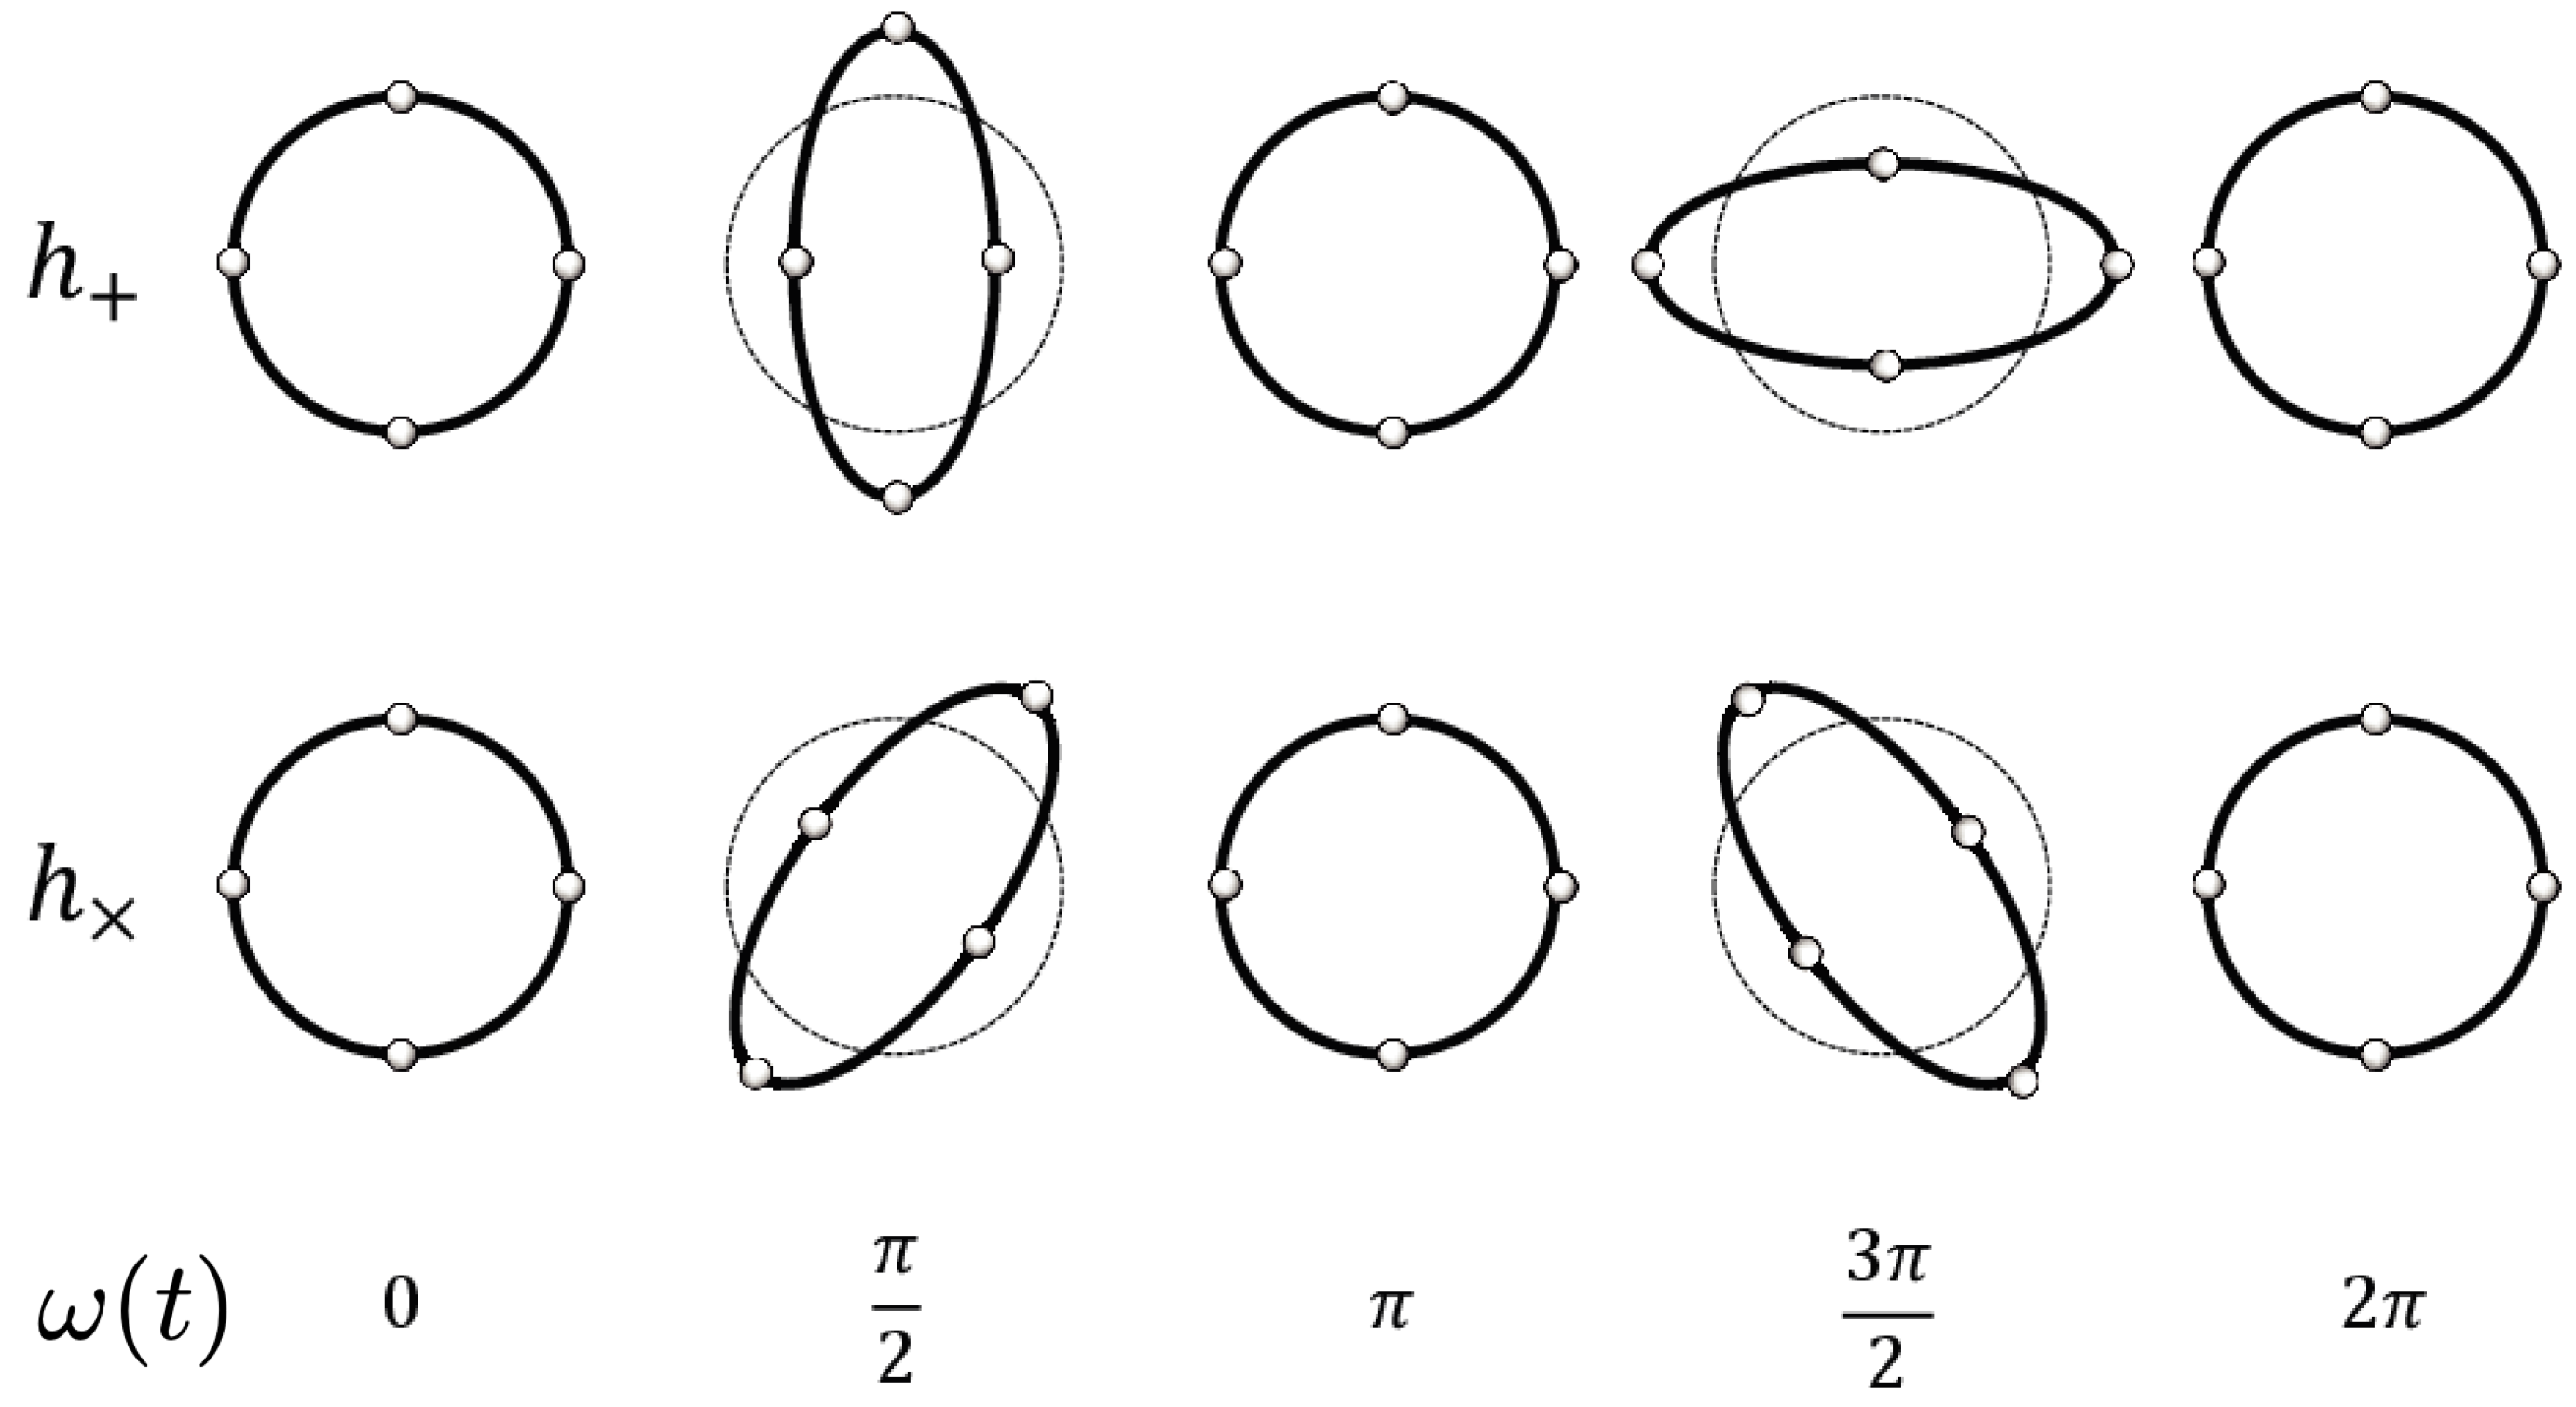
\includegraphics[scale=1]{ring}
		\centering
		\caption{The effects of plus and cross polarization on a ring of test masses. 
			 The plus polarization alternately compresses and stretches the x- and y-separations.
			 The cross polarization has the same effect only rotated by  $\ang{45}$.}
		\label{fig:ring}
		\end{figure}


\section{Energy and momentum of gravitational waves}
	Energy has been one of the most confusing aspects of gravitational wave theory and hence of general relativity.
	The fact that GWs do indeed carry energy and momentum is already clear from the discussion of the interaction of GWs with test masses:
	in the proper detector frame, an incoming GW sets in motion a ring of test masses initally at rest, 
	so GWs impart kinetic energy to these asses.
	If, for example, these masses are connected together with a loose spring with friction, 
	this kinetic energy will be dissipated into heat.
	Conservation of energy requires that the kinetic energy acquired by the test masses must necessarily come from the energy of the GWs.
	The problem is difficult because of the equivalence principle: in a local frame there are no waves and hence no local definition 
	of energy that can be coordinate-invariant.
	Moreover, a wave is a time-dependent metric, and in such spacetimes there is no global energy conservation law. 
	(Recall that conservation laws are associated with symmetry.
	Angular momentum is conserved only in axisymmetric systems, or in systems governed by axisymmetric forces or fields.
	Likewise, energy is conserved on in time-invariant systems.) 
	Energy is only well-defined in certain regimes, which coincide with those for which waves can be cleanly separated from ”background”
 	metrics.


\subsection{Effect of gravitational waves on the background spacetime}

	In order to consider the fact that GWs generate a curvature, the background spacetime has to be dynamical, 
	and this implies that GWs are defined as perturbations over some curved, dynamical, 
	background metric $\bar g_{\mu \nu}$, that is now allowed to be curved and expand in such way

		\begin{equation}
		g_{\mu \nu}(x) = \bar g_{\mu \nu}(x) + h_{\mu \nu}(x) \hspace*{2cm}\|h_{\mu\nu}\|\ll 1
		\end{equation}

	In order to understand how the perturbation $h_{\mu \nu}$ propagates and how it affects the background spacetime, 
	we have to to decide which part of $g_{\mu\nu}$ is the background and which is the fluctuations. 
	Having a dynamical background metric requires a splitting that in linearized theory, 
	having chosen the background metric as the constant flat-space metric $\eta_{\mu\nu}$, was not necessary.

	There is no natural way to do such a split, hence some assumptions are needed: we are considering the situation in which, 
	in some reference frame, we can separate the metric into a background plus fluctuations, 
	and this separation is based on the fact that there is a clear distinction of scales either in space or in time.
	Assuming that in some coordinate system, the $\bar g_{\mu \nu}$ has some typical length scale of spatial variation $L_B$, 
	on top of which small amplitude perturbations are superimposed, characterized by a wavelength $\lambda$ such that $\lambda \ll L_B$. 
	In this case $h_{\mu\nu}$ has the physical meaning of small ripples on a smooth background.
	Equivalently, in a frequency space $\bar g_{\mu\nu}$ has frequencies up to a maximum value $f_b$ and  $h_{\mu\nu}$  
	is peaked around a frequency $f$, with $f >> f_b$.

	First of all, let's expand the Einstein equations around the background $\bar g_{\mu \nu}$ in terms of two small parameters: 
	the typical amplitude $h= O(|h_{\mu\nu}|)$, and either $\lambda/L_B$ or $f_B/f$.
	It is convenient to write the Einstein equations as

		\begin{equation}
		R_{\mu\nu} = {{8\pi G}\over c^4}(T_{\mu\nu}- {1 \over 2}g_{\mu\nu}T) 
		\end{equation}

	where $T_{\mu\nu}$ is the energy-momentum tensor of matter and $T$ its trace.The expantion of the Ricci tensor to $O(h^2)$ is

		\begin{equation}
		R_{\mu\nu} = {\bar R_{\mu\nu}} + R_{\mu\nu}^{(1)} + R_{\mu\nu}^{(2)} + ...
		\end{equation}

	where $ {\bar R_{\mu\nu}}$ is constructed with $\bar g_{\mu\nu}$ only, thus it contains only low frequency modes;
	$R_{\mu\nu}^{(1)}$ is linear in $h_{\mu\nu}$ and it contains high frequency modes;
	and $R_{\mu\nu}^{(2)} $ is quadratic in $h_{\mu\nu}$, it contains both high and low frequency modes.
	Therefore the Einstein equations can be split into two separate equations for the low and high frequency parts

		\begin{equation}
		{\bar R_{\mu\nu}} = -[R_{\mu\nu}^{(2)}]^{Low} + {{8\pi G}\over c^4}(T_{\mu\nu}- {1 \over 2}g_{\mu\nu}T) ^{Low}
		\end{equation}

	and

		\begin{equation}
 		R_{\mu\nu}^{(1)} = - [R_{\mu\nu}^{(2)}]^{High} +  {{8\pi G}\over c^4}(T_{\mu\nu}- {1 \over 2}g_{\mu\nu}T)^{High}
		\end{equation}

	One way to project on the long wavelenght modes is to introduce a scale $\bar l$ such that $\lambda << \bar l << L_B$, 
	and averaging over a spatial volume with side $\bar l$.
	A wavelenght of order $L_B$ is constant over the volume used for the averaging, 
	while modes with a reduced wavelenght of order $\lambda$ are oscillating very fast and average to zero.
	The low-frequency Einstein equations become

		\begin{equation}
 		{\bar R_{\mu\nu}} = - <R_{\mu\nu}^{(2)}> +  {{8\pi G}\over c^4}(T_{\mu\nu}- {1 \over 2}g_{\mu\nu}T) ^{High}
		\end{equation}

	where $<..>$ denotes a spatial average over many reduced wavelenghts, over a volume with sides $l$.
	We now define an effective energy-momentum tensor of matter, $\bar T^{\mu\nu}$

		\begin{equation}
		{\bar T^{\mu\nu}} - {1 \over 2}{\bar g_{\mu\nu}}{\bar T} = <T_{\mu\nu}- {1 \over 2}T>
		\end{equation}

	where ${\bar T}$ is the trace.
	We also define the quantity $t_{\mu\nu}$ as

		\begin{equation}
		t_{\mu\nu} = -{{c^4}\over{8\pi G}}<R_{\mu\nu}^{(2)} - {1 \over 2}{\bar g_{\mu \nu}}R^{(2)}>
		\end{equation}

	whose trace is $t= {\bar g^{\mu\nu}}t_{\mu\nu} = {{c^4}\over{8\pi G}}<R_{\mu\nu}^{(2)}>$.
	Then the low-frequency Einstein equations can be written as

		\begin{equation}
		 {\bar R_{\mu\nu}} = -{1 \over 2}{\bar g^{\mu\nu}} {\bar R} =  {{8\pi G}\over c^4}({\bar T_{\mu\nu}}+t_{\mu\nu})
		\end{equation}

	These equations determine the dynamics of $\bar g_{\mu\nu}$, which is the long-wavelength part of the metric, 
	in terms of the low-frequency part of the matter energy-momentum tensor, $\bar T_{\mu\nu}$, 
	and of a tensor $t_{\mu\nu}$ which does not depend on the external matter but only on the gravitational field itself, 
	and is quadratic in $h_{\mu\nu}$.
	These equations show that the effect of GWs on the background curvature is formally identical to that of matter 
	with energy-momentum tensor $t_{\mu\nu}$, which comes out automatically in an averaged form because 
	one is passing from a microscopic description to a macroscopic one.

















































%--------------------------------------------------------
\section{Gravitational waves vs Electromagnetic waves}
The generation and propagation of gravitational and electromagnetic radiation are basically quite similar but, on a more practical level, gravitational and electromagnetic waves are quite different.
First of all, electromagnetic waves interact strongly with matter; GWs do not.
The weak interaction of GWs means that they propagate from emission to Earth-bound observers with essentially zero absorption, making it possible to probe astrophysics that is hidden or dark to
electromagnetic observations — e.g., the coalescence and merger of black holes, the collapse of a stellar core, the dynamics of the early Universe. It also means that detecting GWs is very difficult.

Electromagnetic radiation typically has a wavelength smaller than the size of the emitting system, and so can be used to form an image of the source.
 This is because electromagnetic radiation is usually generated by moving charges in the environment of some larger source — e.g., an atomic transition in interstellar gas, or emission from hot plasma
 in a stellar environment. By contrast, the wavelength of gravitational radiation is typically comparable to or larger than the size of the radiating source.
GWs are generated by the bulk dynamics of the source itself — e.g., the motion of neutron stars in a binary. As a consequence, GWs cannot be used to form an image: the radiation simply does not
resolve the generating system. Instead, GWs are best thought of as analogous to sound — the two polarizations carry a stereophonic description of the source’s dynamics.

Gravitons in a gravitational-wave burst are phase coherent; photons in electromagnetic signals are usually phase-incoherent. This arises from the fact that each graviton is generated from the same
bulk motion of matter or of spacetime curvature, while each photon is normally generated by different, independent events involving atoms, ions or electrons.
Thus GWs are similar to laser light. We can take advantage of the phase coherence of GWs to enhance their detectability. Matched filtering techniques for detecting GW bursts with well-modeled
functional form (like those generated by coalescing compact binaries) extend the distance to which sources can be seen by a factor of roughly the square root of the number of cycles in the waveform,
a significant gain.

An extremely important consequence of this coherency is that the direct observable of gravitational radiation is the strain $h$, a quantity that falls off with distance as $1/r$.
Most electromagnetic observables are some kind of energy flux, and so fall off with a $1/r^2$ law; measuring coherent GWs is analogous to measuring a coherent, $1/r$
electromagnetic radiation field. This comparatively slow fall off with radius means that relatively small improvements in the sensitivity of GW detectors can have a large impact on their science:
doubling the sensitivity of a detector doubles the distance to which sources can be detected, increasing the volume of the Universe to which sources are measurable by a factor of 8.
Every factor of two improvement in the sensitivity of a GW observatory should increase the number of observable sources by about an order of magnitude.
In most cases, electromagnetic astronomy is based on deep imaging of small fields of view: Observers obtain a large amount of information about sources on a small piece of the sky.
GW astronomy will be a nearly all-sky affair: GW detectors have nearly $4\pi$ steradian sensitivity to events over the sky. A consequence of this is that their ability to localize a source on the sky
 is not good by usual astronomical standards; but, it means that any source on the sky will be detectable, not just sources towards which the detector is “pointed”.
The contrast between the all-sky sensitivity but poor angular resolution of GW observatories, and the pointed, high angular resolution of telescopes is very similar to the angular resolution contrast
 of hearing and sight, strengthening the useful analogy of GWs with sound.
It is useful to categorize GW sources (and the methods for detecting their waves) by the frequency band in which they radiate.
Broadly speaking, we may break the GW spectrum into four rather different bands: the ultra low frequency band,$10^{-18}Hz \apprle f \apprle 10^{-13} Hz$;
the very low frequency band, $10^{-9} Hz \apprle f \apprle 10^{-7} Hz$; the low frequency band, $10^{-5} Hz \apprle f \apprle 1Hz$; and the high frequency band, $1Hz \apprle f \apprle 10^4 Hz$.
iFor compact sources, the GW frequency band is typically related to the source’s size $R$ and mass $M$.
Here the source size $R$ means the lengthscale over which the source’s dynamics vary; for example, it could be the actual size of a particular body, or the separation of members of a binary.
The “natural” GW frequency of such a source is $f_{GW} \sim (1/2\pi)\sqrt{GM/R^3}$. Because $R \apprge 2GM/c^2$ (the Schwarzschild radius of a mass $M$), an upper bound for the frequency of a compact
 source can be estimated:
\begin{equation}
f_{GW}(M) < {1 \over {4\sqrt{2 \pi}}}{{c^3}\over{GM}} \approx 10^4 Hz ({{M_{\odot}} \over M})
\end{equation}
This is a rather hard upper limit, since many interesting sources are quite a bit larger than $2GM/c^2$, or else evolve through a range of sizes before terminating their emission at
 $R \approx 2GM/c^2$. Nonetheless, this frequency gives some sense of the types of compact sources that are likely to be important in each band — for example,
high frequency compact sources are of stellar mass (several solar masses);
low frequency compact sources are thousands to millions of solar masses, or else contain widely separated stellar mass bodies.



\section{High frequency}
The high frequency band, $1Hz \apprle f \apprle 10^4 Hz$, is targeted by the new generation of ground-based laser interferometric detectors such as LIGO.
(It also corresponds roughly to the audio band of the human ear: When converted to sound, LIGO sources are audible to humans.)
The low frequency end of this band is set by the fact that it is extremely difficult to prevent mechanical coupling of the detector to ground vibrations at low frequencies,
and probably impossible to prevent gravitational coupling to ground vibrations, human activity, and atmospheric motions.
The high end of the band is set by the fact that it is unlikely any interesting GW source radiates at frequencies higher than a few kilohertz. Such a source would have to be relatively
low mass $(\apprle 1M_{\odot})$ but extremely compact.There are no known theoretical or observational indications that gravitationally collapsed objects in this mass range exist.
Several interferometric GW observatories are either operating or being completed in the United States, Europe, Japan, and Australia.
Having multiple observatories widely scattered over the globe is extremely important: the multiplicity gives rise to cross-checks that increase detection confidence and also aids in the interpretation
 of measurements. For example, sky location determination and concomitant measurement of the distance to a source follows from triangulation of time-of-flight differences between separated detectors.
\begin{itemize}
  \item LIGO. The Laser Interferometer Gravitational-wave Observatory[55] consists of three operating interferometers:
a single four kilometer interferometer in Livingston, Louisiana, as well as a pair of interferometers (four kilometers and two kilometers) in the LIGO facility at Hanford, Washington.
The sites are separated by roughly 3000 kilometers, and are situated to support coincidence analysis of events.
  \item Virgo. Virgo is a three kilometer French-Italian detector under construction near Pisa, Italy which employs a very sophisticated seismic isolation system that promises extremely good low
frequency sensitivity.
  \item GEO600. GEO600 is a six hundred meter interferometer constructed by a German-English collaboration near Hanover, Germany.
 Despite its shorter arms, GEO600 achieves sensitivity comparable to the multi-kilometer instruments using advanced interferometry techniques.
 This makes it an invaluable testbed for technology to be used in later generations of the larger instruments, as well as enabling it to make astrophysically interesting measurements.
  \item TAMA300. TAMA300 is a three hundred meter interferometer operating near Tokyo.

\end{itemize}


INSERT FIGURE!!!!

The figure shows the detectors sensitivities and "facility limits", the lowest noise levels that can be achieved even in principle within an interferometer facility.
The low level facility limits come from gravity-gradient noise: noise arising from gravitational coupling to fluctuations in the local mass distribution (such as from seismic motions in the earth near
 the test masses,human activity near the detector, and density fluctuations in the atmosphere. At higher frequencies, the facility limit arises from residual gas (mostly hydrogen) in the
interferometer vacuum system — stray molecules of gas effectively cause stochastic fluctuations in the index of refraction.

\section{Low frequency}
There is no hope of measuring GWs in the low frequency band, $10^{-5} Hz \apprle f \apprle 1 Hz$, using a ground based instrument: even if it were possible to completely isolate one’s instrument from
local ground motions, gravitational coupling to fluctuations in the local mass distribution ultimately limits the sensitivity to frequencies $f \apprge 1 Hz$.
Nonetheless, many extremely interesting sources radiate in this band.
The only way to measure these waves is to build a detector in the quiet environment of space, far removed from low-frequency noise sources.
Such an instrument is currently being designed jointly by NASA in the United States and ESA, the European Space Agency: LISA, the Laser Interferometer Space Antenna. LISA will be a laser
interferometer, similar in concept to the ground-based detectors: changes in the distance between widely separated test masses will be monitored for GWs.
However, LISA’s scale is vastly larger than that of its ground-based cousins, and so details of its operations are quite different.
In particular, LISA will have armlengths $L \backsimeq 5 \times 10^6 km$. The three spacecraft which delineate the ends of LISA’s arms are placed into orbits such that LISA forms a triangular
constellation orbiting the sun, inclined $\ang{60}$ with respect to the plane of the ecliptic and following the Earth with a $\ang{20}$ lag.
Since it essentially shares Earth’s orbit, the constellation orbits the sun once per year, “rolling” as it does so.
This motion plays an important role in pinpointing the position of sources by modulating the measured waveform — the modulation encodes source location and makes position determination possible.
The 3 spacecraft each contain two optical assemblies, each of which houses a 1 Watt laser and a 30 centimeter telescope.
 Because of the extreme lengths of the interferometer’s arms, Fabry-Perot interferometry as in the ground-based detectors is not possible:
diffraction spreads the laser beam over a diameter of about 20 km as it propagates from one spacecraft to the other. A portion of that 20 km wavefront is sampled with the telescope.
That light is then interfered with a sample of light from the on-board laser. Each spacecraft thus generates two interference data streams; six signals are generated by the full LISA constellation.
From these six signals, we can construct the time variations of LISA’s armlengths and then build both GW polarizations.
Note that the LISA armlengths are not constant — as the constellation orbits, the distances between the various spacecraft vary by about 1\% (including effects such as planetary perturbations).
These variations are far larger than the displacements produced by GWs, which are of order picometers.
However, these variations occur over timescales of order months, and are extremely smooth and well modeled. It will
 The GW signals are actually read out by monitoring the position of the so- called “gravitational sensor” on each optical assembly; in particular, the position of a “proof mass” which floats freely
 and constitutes the test mass for the LISA antenna is monitored. Because it is freely floating, the proof mass follows a geodesic of the spacetime.
Micronewton thrusters keep the bulk spacecraft centered on these proof masses, forcing the craft to follow their average trajectory.
In this way, the spacecraft are isolated from low frequency forces that could impact the ability to measure GWs (e.g., variations in solar radiation pressure).


\section{GWs Detectors}
As a GW causes the stretching and shrinking of the proper distance between test particles, GWs can be observed by measuring these changes in the proper distance.
The influences of GW is measured by interferometers, that are configured to show destructive interference when no distortions are present.
When a GW passes such a detector, the configuration will no longer support the destructive interference and a bright spot can be seen.
By measuring the intensity of this spot as well as its temporal variation, one will be able to observe the footprints of a GW.

\begin{figure}
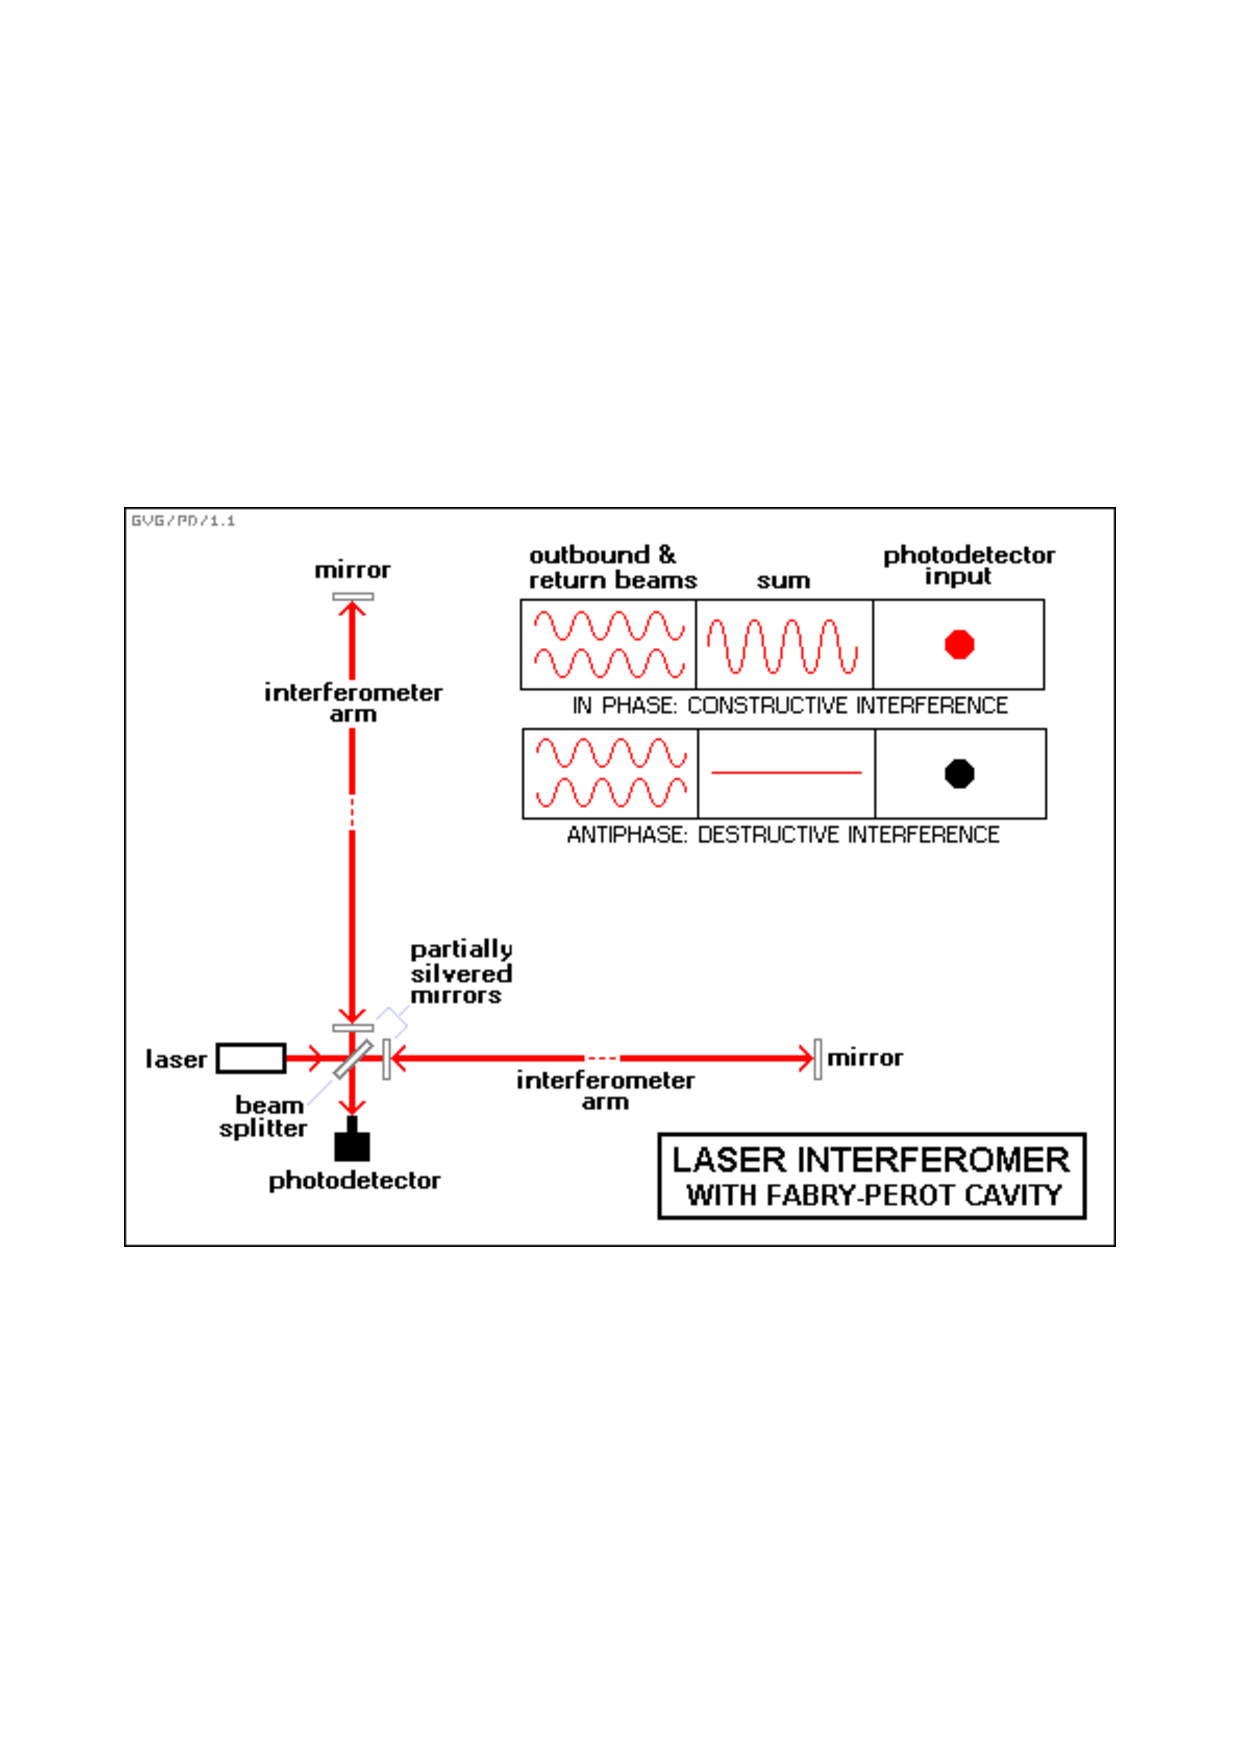
\includegraphics[scale=0.55]{spot}
\centering
\caption{Schematic overview of an interferometric detector. Without a GW present, the interferometer is kept at a destructive interference configuration.
A GW will change the relative distance between the arms and cause the interferometer output to deviate from the destructive interference.
 The intensity of the light and its temporal evolution encode the footprints of GWs.}
\label{fig:spot}
\end{figure}

The first gravitational wave detectors were resonant-mass cylindrical bar detectors. The first was developed and built by Joseph Weber in the 1960s.
Over the course of the next several decades, more bar detectors were built that were at least four orders of magnitude more sensitive than Weber’s original design.
These detectors would be set into oscillation at their resonant frequency by passing gravitational waves near that resonant frequency and were sensitive to gravitational waves with relatively high
 frequency $(\textasciitilde 1 kHz)$ and in a narrow frequency band. In order to detect signals in a broader range of frequencies and out to farther distances, large-scale interferometric detectors
 have been built. The idea originated with the Russian theorists, M. Gertsenshtein and V. I. Pustovoit in 1962. But the strong push for using interferometers came in the late 1960s with
R. Forward, R. Weiss, R. Drever, and others. From the early 2000s, several kilometer-scale ground-based interferometers operated in the frequency band from - 10 Hz to - 1 kHz at a sensitivity that all
owed the potential for detection from a variety of sources at large extragalactic distances.
An interferometric detector is based on the simple principles of a Michelson interferometer. In general, an interferometer uses laser light as a displacement measuring device.
Two highly reflecting mirrors and a central beam splitter (a 50\% reflecting mirror) act as test masses. The three masses are suspended as pendulums and are allowed to swing freely in the horizontal
 direction. Thus, they can be considered freely falling masses in that direction. The reflecting mirrors,  labeled as test masses, are placed equidistant from the central beam splitter but in
orthogonal directions.
A beam of laser light is incident on the beam splitter and is split into two beams along the x and y arms. The light is then reflected by the end mirrors, recombined at the beam splitter,
 and detected at the photodiode. When the beams recombine, they will interfere constructively if the lengths of the two arms differ by an integral number of wavelengths and interfere destructively
if the lengths differ by an odd number of half wavelengths:
%\begin{equation}
%
%\end{equation}


\subsection{Beam pattern functions}

Interferometers are sensitive to the relative difference between two distances, the so-called strain.
 Suppose we have an interferometer with its arms pointing along the unit vectors $u^i$ and $v^i$. The strain $h(t)$ is given by
\begin{equation}
h(t) = {1 \over 2} (h_{ij}u^iu^j - h_{ij}v^iv^j) = D^{ij}h_{ij}(t)
\end{equation}
where $D^{ij}$ is referred to as the detector tensor and is given by
\begin{equation}
D^{ij} = {1\over 2} (u^iu^j -v^iv^j)
\end{equation}
As the expression for $h(t)$ is linear in $h_{+}$ and $h_{\times}$, one can also write
\begin{equation}
h(t) = F_{+}h_{+} (t) + F_{\times}h_{\times}(t)
\end{equation}
where $F_{+,\times}$ are called the beam pattern functions. Suppose we have a detector with arms that are perpendicular to each other, one pointing in the x-direction and the other
in the $y$-direction in a Cartesian coordinate system. This detector frame, denoted by $(x,y,z)$, is generally different from the GW coordinate system, denoted by $(x^\prime,y§^\prime,z^\prime)$, where the source
is conveniently described. To account for such a difference, we first note that when the plus and cross polarisations are not equal in strength, we can rotate the coordinate system by
an angle $\psi$ around the $z^\prime$ axis so that the $x^\prime$ and $y^\prime$ axes coincide with the mayor and minor axis of the associated ellipse.
 In going from the GW frame to the detector frame, we can rotate the GW frame by an angle $\theta$ around the $x^\prime$ axis and an angle $\phi$ around the $z^\prime$ axis,
where the angles $(\theta, \phi)$ denote the direction of propagation of the GW in the detector frame.
Applying these three rotations, the beam pattern functions for a detector with perpendicular arms are given by 
\begin{align}
F_{+}^{\ang{90}}& = {1 \over 2} (1 + \cos^2 \theta)\cos 2\phi \cos 2 \psi - \cos \theta \sin2\phi \sin2\psi \\
F_{\times}^{\ang{90}}& = {1 \over 2} (1 + \cos^2 \theta)\cos 2\phi \sin 2 \psi + \cos \theta \sin2\phi \cos2\psi
\end{align}

\subsection{The Noise Spectral Density}
The various noises of the detector can be conveniently characterized by a spectral strain
sensitivity with dimensions of $1/sqrt{Hz}$. 
The the detector output $s(t)$ is composed of instrumental noise $n(t)$ arising from naturally occurring random processes and a potential strain signal $h(t)$
\begin{equation}
s(t) = n(t) + h(t)
\end{equation}

The detection problem then becomes how to distinguish $h(t)$ from $n(t)$ when $h(t) << n(t)$. In a way, $n(t)$ provides a measure of how small an $h(t)$ we can detect. Thus we take $n(t)$ as the
detector’s noise and have a convenient way to compare performances of different detectors. Instrumental noise is a random process. In the case that we have a stationary random process (which can be the case for detector noise for short periods of time), the expectation value of $n$ at some time t becomes a long time average (as opposed to an ensemble average):
\begin{equation}
<n> = \lim_{T \to \infty} {1 \over T} \int^{T/2}_{-T/2}n(t)dt
\end{equation}
For simplicity, let us assume that $<n> = 0$. We can still define the power in the signal by integrating $n^2(t)$ over some duration $T$ and then dividing by $T$. Again, the expectation value of $n^2(t)$ will just be the time average:
\begin{equation}
<n^2> = \lim_{T \to \infty} {1 \over T} \int^{T/2}_{-T/2}n^2(t)dt
\end{equation}
If $n(t) = 0$ outside of $−T/2 < t < T/2$, then we can extend the integral limits to infinity 
\begin{equation}
\begin{split}
  <n^2>  = \lim_{T \to \infty}{1 \over T}int^{\infty}_{-\infty}n^2(t) dt \\
         = \lim_{T \to \infty}{1 \over T} \int^{\infty}_{-\infty}|\~{n}(f)|^2df \\ 
         = \lim_{T \to \infty}{2 \over T} \int^{\infty}_{0}|\~{n}(f)|^2df \\
         = \int^{\infty}_{0}S_n(f)df
\end{split}
\end{equation}
where $S_n$ is what is known as the power spectral density of the noise process $n(t)$ and $\~{n}(f)$ is the Fourier transform of $n(t)$. Thus, in general, the power spectral density of a stationary random process $n(t)$ is defined as
\begin{equation}
= \lim_{T \to \infty}{2 \over T} |\int^{T/2}_{-T/2}n(t)e^{-2\pi ift}dt|^2
\end{equation}
Another useful expression for the power spectral density can be found by finding the expectation value of the frequency components of the noise

\begin{equation}
<\~{n}\ast(f\prime)\~{n}(f)>  = {1 \over 2} S_n(f) \delta (f-f\prime)
\end{equation}

Since the noise is real, $\~{n}(-f) = \~{n}(f)$ and thus, $S_n(−f) = Sn(f)$. If $n(t)$ has no dimensions, then $S_n(f)$ has units of $Hz^{-1}$.
 If $<\~{n}\ast(f\prime)\~{n}(f)> $ is obtained by integrating only over the physical
range of frequencies, $f > 0$, then $S_n(f)$ is known as the $one-sided spectral density$.
Finally, on further definition that will come in handy is the inner product of $a$ and $b$:


\begin{equation}
(a|b) = 2 \int^{\infty}_{-\infty} {{\~{a}(f)\~{b}\ast()f} \over {S_n(f)}}df = 4 Re [\int^{\infty}_{0}{{\~{a}(f)\~{b}\ast(f)} \over {S_n(f)}} df]
\end{equation}

\subsection{Dominant Noise Sources}
The three dominant noise sources for the initial detectors were seismic, thermal, and shot noise.

$Photon Shot Noise$
The primary limitation in measuring a small change in light is shot noise, or the natural fluctuations in the rate of photons arriving at the photodiode, that follow a Poisson process. The noise will decrease with increasing laser power, recycling cavity gain, arm cavity gain, and arm length.

$Radiation Pressure Sensor Noise$
Radiation pressure noise is associated with the photons from the laser striking the mirror and causing a force on the mirror. Of course, increasing the laser power to combat shot noise will actually result in an increase of radiation pressure. This noise source dominates the sensor noise at low frequencies while shot noise dominates at high frequencies. Thus one must optimize the laser power to give the smallest sensor noise overall.
 
$Seismic Noise$
At low frequencies, below about 40 Hz for initial LIGO, ground motion is the dominant
source of noise. It shakes the optics and produces strain signals that mask gravitational wave
signals. It would actually dominate at higher frequencies as well if it were not for a series
of active- and passive-isolation systems. The first line-of-defense is suspending the optics
as pendulums. For ground-motion frequencies much larger than the pendulum frequency
($f_{pend} = 0.76 Hz$ for initial LIGO), motion of the optics will be suppressed. Further sup-
pression occurs from four alternating mass-spring layers which provide an attenuation factor
$\propto f^{-2}$.

$Thermal Noise$
At frequencies of about 40-100 Hz, the random Brownian motion of the molecules on the surface of the mirrors and wires dominates. Initial LIGO’s two most important sources of thermal noise are the pendulum suspension system and the internal vibration modes of the mirrors.

$Gravity Gradient Noise$
ravity gradient noise is actually due to the gravitational attraction between the test masses and density fluctuations in the atmosphere and earth in the local vicinity of the detector. It was not a dominant source of noise for initial detectors but will be for advanced detectors at low frequencies.


\subsection{Sources}

\subsection{Coalescing compact binaries}
Compact binaries — binary star systems in which each member is a neutron star or black hole — are currently the best understood sources of GWs.
 Double neutron stars have been studied observationally since the mid 1970s; five such systems tight enough to merge within a few 108 or 109 years have been identified in our Galaxy.
Extrapolation from these observed binaries in the Milky Way to the Universe at large indicates that GW detectors should measure at least several and at most several hundred binary neutron star mergers
 each year (following detector upgrades; the expected rate for initial detectors is of order one event per several years, so that measurement of an event is plausible but of fairly low probability).
Population synthesis (modelling evolution of stellar populations) indicates that the measured rate of binaries containing black holes should likewise be interestingly large (perhaps even for initial
 detectors). The uncertainties of population synthesis calculations are rather large, however, due to poorly understood aspects of stellar evolution and compact binary formation;
 data from GW detectors is likely to have a large impact on this field.

\subsection{Stellar core collapse}
Core collapse is likely to be an important source of GWs, it exhibits all of the necessary conditions for strong GW generation: large amounts of mass (1 - 100 $M_{\odot}$) flow in a compact region
 (hundreds to thousands of kilometers) at relativistic speeds (v/c $\apprge$ 1/5). However, these conditions are not sufficient to guarantee strong emission.
In particular, the degree of asymmetry in collapse is not particularly well understood.
If the core of a star is very rapidly rotating during collapse, then instabilities may develop which lead to strong GW emission.
If such instabilities develop, core collapse GWs could be detected from events as far away as 10 Megaparsecs, a distance encompassing enough galaxies that several events per year would be likely.
Most models of massive stars, however, indicate that such rapid rotation is not likely.
Even without the growth of instabilities, the asymmetric dynamics of core collapse is likely to lead to wave emission which would be detectable within the Local Group of galaxies, with perhaps an
event every few years detectable by advanced interferometers.
The wave strength is likely to correlate strongly with the degree of asymmetry in the supernova.
If the GW event has an electromagnetic or neutrino counterpart we may gain a wealth of knowledge regarding the state of the precollapse core.

\subsection{Continuous Sources}
A source that emits gravitational waves for a long period of time (typically more than a few minutes, oftentimes much more than a year) is known as a continuous gravitational wave source. Such sources would typically be high frequency rotating neutron stars with a non-axial deformation or low frequency binary systems composed of white dwarfs or black holes far from merger. Typically, these sources can be modeled by nearly fixed frequency sinusoids.
In the high frequency regime, rapidly rotating, distorted neutron stars could be a source of high frequency gravitational waves. Very simply, we could model such a system as a rotating triaxial ellipsoidal bar spinning about its $z$-axis, principal axis of inertia $I_3$. We can assume that the quadrupole tensor is diagonal at $t = 0$ and that the bar is spinning with angular velocity $\omega$; but for an observer at an inclination angle, we need to rotate the second time derivative of the quadrupole tensor, take the TT projection and compute the gravitational wave perturbation.

\subsection{Periodic emitters}
Periodic sources of GWs radiate at constant or nearly constant frequency, like radio pulsars.
In fact, the prototypical source of continuous GW is a rotating neutron star, or GW pulsar. A non-axisymmetry in a neutron star crust (caused, for example, by an oblateness that is misaligned with
the star’s spin axis) will radiate GWs with characteristic amplitud
\begin{equation}
 h \sim {G \over c^4}{{If^2\epsilon}\over{r}}
\end{equation}
Here $I$ is the star's moment of inertia, $f$ is the wave frequency, $r$ is the distance to the source, and $\epsilon$ is the dimensionless fractional distortion $\epsilon = (I_{xx}-I_{yy})/I$,
where $I_{ij}$is the moment of inertia tensor. The crucial parameter $\epsilon$ characterizes the degree to which the star is distorted; it is rather poorly understood.
Upgraded interferometers in LIGO could set an upper limit on  $\epsilon$ of order $10^{-6}$ for sources at $\sim10$ kpc.
Various mechanisms have been proposed to explain how a neutron star can be distorted to give a value of $\epsilon$hat is interesting as a GW source.
Whatever the mechanism generating the distortion, it is clear that  $\epsilon$ will be small,
so that $h \sim 10^{-24}$or smaller — quite weak. Measuring these waves will require
coherently tracking their signal for a large number of wave cycles. Coherently tracking $N$ cycles boosts the signal to noise ratio by a factor $\sim sqrt{N}$.
his is actually fairly
 difficult, since the signal is strongly modulated by the Earth’s rotation and orbital
motion, “smearing” the waves’ power across multiple frequency bands. Searching for
periodic GWs means demodulating the motion of the detector, a computationally
intensive problem since the modulation is different for every sky position. Unless
one knows in advance the position of the source, one needs to search over a huge number of sky position "error boxes", perhaps as many as $10^13$.
As mentioned above, one particularly interesting mechanism for distorting a neutron star comes from accretion of material from a companion star. Accretion provides a spin-up torque to a neutron star,
\begin{equation}
(dJ/dt)_{spin-up} \sim R^2\Omega_* \dot M
\end{equation}
(where $J$  is the spin angular momentum, $\Omega_* $ is the orbital frequency of the accreting matter as it pulunges onto the star, $R$ is the star's radius , and $\dot M$
is the mass accretion rate).
Without any kind of braking mechanism, the neutron star would presumably spin-up until it reaches the “breakup limit”, i.e., the spin frequency at which centrifugal forces would begin to break it
apart; the breakup frequency is typically around 2000 – 3000 Hz.

Observations have shown that accreting neutron stars do, in fact, appear to have a “speed limit” — no accreting neutron star has been observed to spin faster than 619 Hz.
This suggest that some mechanism is removing angular momentum from the neutron star.
A plausible and very attractive possibility for how this angular momentum is removed is via GW emission. Because the spin-down torque
due to GW emission grows sharply with spin frequency,
\begin{equation}
(dJ/dt)_{spin-up} \propto \Omega^5 
\end{equation}
the limiting spin obtained by balancing the torquess relatively insensitive to the mass accretion rate $\dot M$.
Whatever the mechanism, accreting neutron stars are obvious and very attractive targets for observing campaigns with GW detectors, particularly given that their sky positions are well known.




\subsection{Stochastic backgrounds}
Stochastic backgrounds are “random” GWs, arising from a large number of independent, uncorrelated sources that are not individually resolvable.
A particularly interesting source of stochastic waves is the dynamics of the early Universe, which could produce an all-sky GW background, similar to the cosmic microwave background.
Stochastic waves can be generated in the early Universe via a variety of mechanisms: amplification of primordial fluctuations in the Universe’s geometry via inflation, phase transitions as previously
unified interactions separate, a network of vibrating cosmic strings, or the condensation of a brane from a higher dimensional space.
These waves can actually extend over a wide range of frequency bands; waves from inflation in particular span all bands, from ultra low frequency to high frequency.
 Stochastic backgrounds are usually idealized as being stationary, isotropic and homogeneous. They are thus characterized by their energy density per unit frequency, $d\rho_{gw}/df$.
This is often parameterized in terms of the energy density per unit logarithmic frequency divided by the critical energy density to close the Universe
\begin{equation}
\Omega_{gw}(f) = {1 \over {\rho_{crit}}}{{d\rho_{gw}}\over{d\ln{f}}}
\end{equation}
where $\rho_{crit} = 3H_0^2/8\pi G$ is the critical densty and $H_0$ is the value of the Hubble constant today.
 Different cosmological sources produce different levels of $\Omega_{gw}(f)$, centered in different bands.
In the high frequency band, waves produced by inflation are likely to be rather weak: estimates suggest that the spectrum will be flat across LIGO’s band,
with magnitude $\Omega_{gw} \sim 10^{-15}$ at best.
Waves from phase transitions can be significantly stronger, but are typically peaked around a frequency that depends on the temperature T of the phase transition
\begin{equation}
f_{peak} \sim 100Hz({T \over {10^5 Tev}})
\end{equation}

Because of their random nature, stochastic GWs look just like noise.
Ground- based detectors will measure stochastic backgrounds by comparing data at multiple sites and looking for “noise” that is correlated.
For comparing to a detector’s noise, one should construct the characteristic stochastic wave strain,
\begin{equation}
h \propto f^{-3/2}sqrt{\Omega_{gw}(f)\Delta f}
\end{equation}
where $\Delta f$ is the frequency band across which the measurement is made.
If $\Omega_{gw}(f)$ is constant, this strain level grows sharply with decreasing frequency — the most interesting limits are likely to be set by measurements at low frequencies.
Early detectors will have fairly poor sensitivity to the background, constraining it to a level $\Omega_{gw} \sim 5 \times 10^{-6}$ in a band from about 100 Hz to 1000 Hz.
This is barely more sensitive than known limits from cosmic nucleosynthesis.





\chapter{Gravitational waves in linearized gravity}

\subsection{Weak-field metric}


In 1915, Albert Einstein presented his general theory of relativity  which describes how mass distorts spacetime and in turn how spacetime dictates how masses flow through it. 
The classical Newtonian notion of gravity ,which stated that gravity arises from an action at a distance, was replaced with a geometric interpretation of the Universe, the spacetime continuum: it 
can be regarded as a fabric and it can be curved by the mass of an object. Masses moving on this curved spacetime fabric will then be perceived as gravity. 
In general relativity, space-time is regarded as a four-dimensional manifold with a Lorentzian metric, and gravity is a manifestation of the manifold’s curvature.
 The spacetime curvature is associated with the stress-energy tensor of matter fields through the Einstein’s field equations:

\begin{equation}
G_{\mu\nu} \equiv R_{\mu\nu}  - {1 \over 2}g_{\mu\nu}R = {8\pi G_{N} \over {c^4}}T_{\mu\nu} 
\end{equation}

Where $G_{\mu\nu} $ is the Einstein tensor, $T_{\mu\nu} $ is the stress-energy tensor of matter-fields and $ G_{N}$ is Newton’s gravitational constant. 

General relativity predicts that gravity is mediated by a new type of radiation: gravitational radiation. 
In 1916 Einstein found the weak-field solutions to general relativity had wave-like solutions, gravitational waves. 
Gravitational waves that compose gravitational radiation are ripples in the fabric of spacetime, which periodically lengthen and shorten space, and speed up and slow down time. 
 To study the properties of gravitational waves, it is instructive to first study them in situations where the gravitational fields are weak. 
In the so-called weak-field approximation, one can view the metric as the Minkowski metric with a small perturbation: it is required to expand the Einstein equations around the flat-space metric, 
considering as a perturbation on the space-time of special relativity. 
Letting $ x_\mu = (t, x, y, z)$ denote the time and space coordinates, we can write the proper distance between events $x_{\mu}$ and
$x_{\mu} + dx_{\mu}$ as
\[
ds^2 = g_{\mu\nu}dx^{\mu}dx^{\nu} \approx (\eta_{\mu\nu} + h_{\mu\nu})dx_{\mu}dx_{\nu}. \hspace*{2cm}\|h_{\mu\nu}\|\ll 1
\]
Here $\eta_{\mu\nu} = diag(-1,1,1,1)$ is the usual Minkowski metric and
 $h_{\mu\nu}$ represents the linearised gravitational field.
The metric perturbation is referred to as  $h_{\mu\nu}$: it encapsulates gravitational waves, but contains additional, non-radiative degrees of freedom as well; $\|h_{\mu\nu}\|$ means 
“the magnitude of a typical non-zero component of $h_{\mu\nu}$”. The condition $\|h_{\mu\nu}\|\ll 1$ requires both the gravitational field to be weak, and in addition constrains the 
coordinate system to be approximately Cartesian.  In linearized gravity, the smallness of the perturbation means that only terms which are linear in $h_{\mu\nu}$ are considered; 
higher order terms are discarded. As a consequence, indices are raised and lowered using the flat metric. 
The metric perturbation $h_{\mu\nu}$ transforms as a tensor under Lorentz transformations, but not under general coordinate transformations: since the numerical values of the components 
of a tensor depend on the reference frame, there exists a reference frame where the linearisation of the gravitational field holds on a sufficiently large region of the spacetime. 
The Einstein field equations are covariant under general coordinate transformations
\begin{equation}
x^{\mu} \rightarrow x^{\mu ‘}(x)
\end{equation}
So that the metric transforms as 
\begin{equation}
g_{\mu\nu} \rightarrow g_{\mu' \nu'} = x^{\rho},_{\mu'}x^{\sigma},_{\nu'}g_{\rho \sigma}
\end{equation}
This means that one is free to choose a convenient coordinate system without altering the physical predictions of the field equations. 
Choosing a reference frame breaks the invariance of general relativity under coordiante trasformations but it also erases spurious degrees of freedom.
However,after choosing a frame where the field is linearised, a residual gauge symmetry remains. Under infinitesimal coordinate transformations
 $x_{\mu} \rightarrow x_{\mu} + \xi_{\mu}$:

Using the transformation law of the metric, to lowest order $h_{\mu\nu}$ transforms as
\[
h_{\mu\nu} \rightarrow h_{\mu\nu} - \partial_{\mu}\xi_{\nu} - \partial_{\nu}\xi_{\mu}
\]





\subsection{Linearising the Einstein field equations}
All the fundamental quantities in the field equations need to be computed in order to linearise the theory. 
Rather than working with the metric perturbation, changing notation and using the trace-reversed perturbation makes the computation more compact and cleaner. Defining 
\begin{equation}
{\bar h}_{\mu\nu} = h_{\mu\nu} - {1 \over {2}}\eta_{\mu\nu}h  
\end{equation}
and the trace 
\begin{equation}
h = \eta^{\mu\nu}h_{\mu\nu}
\end{equation}
expressing the trace-reversed field:
\begin{equation}
h_{\mu\nu} = {\bar h}_{\mu\nu} + {1 \over {2}}\eta_{\mu\nu}{\bar h}
\end{equation} 
The Rienmann tensor constructed in linearised theory is given by
\begin{align}
R^{\mu}{\nu\rho\sigma} = \partial_{\rho} \Gamma^{\mu}_{\nu\sigma} - \partial_{\sigma}\Gamma^{\mu}_{\nu\rho}  \\
&={ 1 \over 2} (\partial_{\rho}\partial_{\nu}h^{\mu}_{\nu\rho} + \partial_{\sigma}\partial^{\mu}h^{\nu\rho} - \partial_{\rho}\partial^{\mu}h^{\nu\sigma} - \partial_{\sigma}\partial_{\nu}h^{\mu}_{\rho})
\end{align}
From this, the Ricci tensor takes the form
\begin{equation}
R_{\mu\nu} = R^{\rho}_{\mu\rho\nu} = {1 \over 2}(\partial_{\rho}\partial{\nu}h^{\rho}_{\mu} + \partial^{\rho}\partial_{\mu}h_{\nu\rho} - \square h_{\mu\nu} - \partial_{\mu}\partial_{\nu}h)
\end{equation}
The curvature scalar is obtained contracting once more:
\begin{equation}
R = R^{\mu}_{\mu} = (\partial_{\rho}\partial^{\mu}h^{\rho}_{\mu} - \square h)
\end{equation}

Combining all together the Einstein tensor can be expressed as
\begin{equation}
G_{\mu\nu} = {1 \over 2}(\partial_{\rho}\partial{\nu}h^{\rho}_{\mu} + \partial^{\rho}\partial_{\mu}h_{\nu\rho} - \square h_{\mu\nu} - \partial_{\mu}\partial_{\nu}h - \eta_{\mu\nu}\partial_{\rho}\partial^{\sigma}h^{\rho}_{\sigma} + \eta_{\mu\nu}\square h)
\end{equation}
Substituting the metric perturbation $h_{\mu\nu}$  with the $trace-reversed$ perturbation ${\bar h}_{\mu\nu}$ and expandig, the linerised Einstein equations assume the  compact form:
\begin{equation}
\square {\bar h}_{\mu\nu} + \eta_{\mu\nu}{\partial}^{\rho}{\partial}^{\sigma}{\bar h}_{\rho\sigma} - {\partial}^{\rho}{\partial}^{\nu}{\bar h}_{\mu\rho} - {\partial}^{\rho}{\partial}^{\mu}{\bar h}_{\nu\rho} = - {{16\pi G_{N}} \over {c^4}}T_{\mu\nu}.
\end{equation}


The linearised equations of motion are gauge-invariant, and the gauge freedom can
 be used to simplify the form of the field equations.
 In the Lorentz family of gauges, choosing the harmonic gauge 
 $ \partial_{\mu}h_{\mu\nu} = 0 $ 
 , reduces the Einstein equations to a simple wave equation that relates the trace-reversed field
 to the stress energy tensor:
\begin{equation}
\square {\bar h}_{\mu\nu} =({\partial^2 \over {\partial t^2} } - {\partial^2 \over {\partial x^2}}  - {\partial^2 \over {\partial y^2}}  -  {\partial^2 \over {\partial z^2}}) {\bar h}_{\mu\nu} = -{{16\pi G_{N}} \over {c^4}}T_{\mu\nu}. 
\end{equation}
By imposing the harmonic gauge one has chosen the coordinates in such a way that for a single plane wave (or a superposition of plane waves with their wave vectors pointing in the same direction), 
the GW polarisations are perpendicular to the direction of propagation.

The harmonic gauge gives four conditions, that reduce the 10 indipendent component of the symmetric 4x4 matrix $h_{\mu\nu}$ to six indipendent component, so it does not fix the gauge completely, 
leaving 4 additional components free to be gauge-fixed.  
If the metric perturbation is not in the harmonic gauge, by making an infinitesimal coordinate transformation 
\begin{equation}
{\bar h}_{\mu\nu} \rightarrow {\bar h}_{\mu’\nu’}  = {\bar h}_{\mu\nu}  - \xi_{\mu,\nu} -\xi_{\nu,\mu} + \eta_{\mu\nu}\xi^{\rho}_{,\rho}
\end{equation}
and applying the harmonic gauge condition

\begin{equation}
{\bar h}_{\mu’\nu’,} ^{\nu’} = {\bar h}_{\mu\nu,} ^{\nu} - \xi_{\mu,\nu}^{\nu}
\end{equation}

Therefore any metric perturbation can be put into an harmonic gauge by making an infinitesimal coordinate transformation that satisfies 
\begin{equation}
{\bar h}_{\mu\nu,} ^{\nu} = \xi_{\mu,\nu}^{\nu}
\end{equation}

This is a wave equation that always admits a solution, thus one can always achieve the harmonic gauge. 
Outside the source where $T_{\mu\nu} = 0$ 

\begin{equation}
\square {\bar h}_{\mu\nu} = 0
\end{equation}

In vacuum spacetimes which are asymptotically flat ($h_{\mu\nu} \rightarrow 0 as r \rightarrow 0$), along with choosing the harmonic gauge, the metric perturbation can be greatly simplified using 
the residual gauge freedom within the harmonic gauge class. The transverse-traceless gauge,  $TT$-gauge, can be obtained by choosing the components of the metric tensor $h_{\mu\nu}$, 
so that only the ones on the plane orthogonal to the direction of propagation (transverse) are different from zero, this results in $h_{\mu\nu}$ being traceless:

\begin{equation}
h^{0\mu} = 0 \hspace*{0.5cm}  h^{i}_i = 0  \hspace*{0.5cm}   {\partial}^jh_{ij} = 0
\end{equation}

By imposing the harmonic gauge, the 10 degrees of freedom of the symmetric matrix $h_{\mu\nu}$ have reduced to six degrees of freedom, and the residual gauge freedom, 
associated to the four functio $\xi^{\mu}$, has further reduced these to just two degrees of freedom, which corrispond to the two possible polarization states of the gravitational wave. 
Equation (1.16) has plane wave solutions, $h_{\mu\nu}^{TT}(x)=e_{ij}(k)e^{ikx}$ with $k^{\mu}=(w/c,k)$ and $w/c=|k|$. The tensor $e_{ij}(k)$ is called the polarization tensor. 
In vacuum spacetimes, a plane gravitational wave with a given wave-vector $k$ is characterized by two functions $h_+$ and $h_{\times}$, while the remaining components can be set to zero by 
choosing the transverse-traceless gauge. Choosing $n$ along the z axis:

\begin{equation} 
h_{\mu\nu}^{TT} = 
\begin{bmatrix}
0 & 0 & 0 & 0 \\
0 & h_{+} & h_{\times} & 0 \\
0 & h_{\times} & -h_{+} & 0 \\
0 & 0 & 0 & 0 
\end{bmatrix}cos[w(t-z/c)]
\end{equation}




\chapter{Interaction of Gravitational waves with test masses}

To understand how gravitational waves interact with the detectors, mirrors in the case of the interferometric detectors, it's necessary to use the geodesic equation and 
the geodesic deviation equation, which are also important tools for understanding the physical meaning of a given gauge choice. 
In fact the physics must be invariant under coordinate trasformations but GWs and the detector description's depend on the chosen reference frame. 


\section{Geodesic equation and geodesic deviation}
The usual notion of “gravitational force” disappears in general relativity, replaced instead by the idea that freely falling bodies follow geodesics in spacetime. 
Geodesics are the curved-space equivalents of straight lines, which can be found by parallel transporting the tangent vector of a curve.
Given a spacetime metric $g_{\mu\nu}$ and a set of spacetime coordinates $x^{\mu}$, geodesic trajectories are given by the equation: 
\begin{equation}
{{d^2x^{\mu}}\over{d\tau^2}} + \Gamma_{\nu\rho}^{\mu}(x){{dx^{\nu}}\over{d\tau}}{{dx^{\rho}}\over{d\tau}} = 0 \hspace*{2cm} m \neq 0
\end{equation}
\begin{equation}
{{d^2x^{\mu}}\over{d\lambda^2}} + \Gamma_{\nu\rho}^{\mu}(x){{dx^{\nu}}\over{d\lambda}}{{dx^{\rho}}\over{d\lambda}} = 0 \hspace*{2cm} m = 0
\end{equation}
which is the classical equation of motion of a test mass in the curved background described by the metric $g_{\mu\nu}$, in the absence of external non gravitational force and where $m$ is the mass 
of the object, $\tau$ represents the proper time given by $d\tau^2 = -ds^2$, and $\lambda$ is some affine parameter on the geodesic. 
In a flat spacetime, two straight lines taht are initially parallel to each other will remain parallel. In a curved spacetime, geodesics do not satisfy this property. 
Instead, two nearby geodesics, separeted by $\zeta^{\mu}$, follow the geodesic deviation equation
\begin{equation}
{{D^2\zeta^{\mu}}\over{D\tau^2}} = -R^{\mu}_{\nu\rho\sigma}\zeta^{\rho}{{dx^{\nu}}\over{d\tau}}{{dx^{\sigma}}\over{d\tau}}
\end{equation}
where $D/D\tau$ is defined as 
\begin{equation}
{{DV^{\mu}}\over{D\tau}} \equiv {{dV^{\mu}}\over{dtau}} + \Gamma^{\mu}_{\nu\rho}V^{\nu}{{dx^{\rho}}\over{d\tau}}
\end{equation}
and denotes the covariant derivative along a curve that is parameterised by $\tau$. The geodesic deviation equation describes the change in separation $\zeta^{\mu}$ between two nearby geodesic. 
As the Rienmann tensor describes the tidal forces caused by the gravitational field, the geodesic deviation equation shows that these tidal forces can be considered as deviations of nearby geodesics.



\subsection{Transverse-traceless gauge}

Consider a test mass initially at rest at $\tau = 0$. The geodesic equation then becomes
\begin{equation}
{{dx^i}\over{d\tau^2}} = -[\Gamma^i_{\nu\rho}{{dx^{\nu}}\over{d\tau}}{{dx^{\rho}}\over{d\tau}}]_{\tau=0} \\ 
= - [ \Gamma^i_{00}({{dx^0}\over{d\tau}})^2]_{\tau=0}
\end{equation}
by assumption
\begin{equation}
{{dx^i}\over{d\tau}} = 0 \hspace*{2cm} at \hspace*{0.5cm}\tau = 0
\end{equation}
since the mass is initially at rest. Expanding to first order in $h_{\mu\nu}$, the Christoffel symbol $\Gamma^i_{00}$ vanishes in the TT gauge
\begin{equation}
 \Gamma^i_{00} = {1 \over {2}}(2\partial_{0}h_{0i} - \partial_i h_{00})
\end{equation}
because both $h_{00}$ and $h_{0i}$ are set to zero by the gauge condition. Therefore, if at time $\tau = 0$ $dx^i/d\tau$ is zero, remains zero at all times, because its derivatives also vanishes. 
This shows that if two test masses are initially separated by a coordinate separation of $x^i$ in the TT frame, and are at rest with respect to each other, they will remain at this separation. 
Overall, it seems that a GW has no influence on the geodesic or on the deviation of geodesics. 
In other words, in the TT gauge the coordinate location of a slowly moving, freely falling body is unaffected by the GW because the coordinates move with the waves.
The TT gauge illustrates that, in general relativity, the physical effects are not expressed by what happens to the coordinates since the theory is invariant under coordinate transformations:
 the position of test masses doesn't change because the freedom of gauge allowed to define the coordinates in such a way that they don't change. 
Physical effects can instead be found monitoring proper distances, or proper times. 

In fact the GWs cause the
proper separation between two freely falling particles to oscillate, even if the coordinate
separation is constant. Consider two spatial freely falling particles, located at $z = 0$, and separated on the x axis by a coordinate distance $L_c$. Consider a GW in TT gauge that propagates down the z axis, $h^{TT}_{\mu\nu}(t,z)$. The proper distance L between the two particles in the presence of the GW is given by
\begin{align}
L & = \int^{L_c}_{0}{dx\sqrt{g_{xx}}} = \int^{L_c}_{0}dx\sqrt{1 + h^{TT}_{xx}(t,z=0)} \\
 & \simeq \int^{L_c}_{0}{dx[1 + {1 \over 2}h^{TT}_{xx}(t,z=0)]} \\
&= L_c[1 + {1 \over 2}h^{TT}_{xx}(t,z=0)]
\end{align}
Therefore, the proper distance expands and shrinks periodically,with a fractional length change $\delta L/L$ given by
\begin{equation}
{{\delta L}\over{L}} \simeq {1 \over 2} h_{xx}^{TT}(t,z=0)
\end{equation}
Even though this result is calculaterd in the TT gauge, it is indeed gauge indipendent.
$h_{xx}^{TT}$ acts as a strain, a fractional length change.
 Because the time that light travels between the two test masses is related to the proper distance,  which directly relates to the accumulated phase measured by laser interferometric GW observatories,
 GWs leave an imprint on the time it takes for a photon to make a round trip. Consequently, interferometers can potentially measure these imprints by measuring the length difference between 
their arms. The “extra” phase $\delta \phi$ (if $L \ll \lambda$ so that the metric perturbation does not change value very much during a light travel time) accumulated by a photon that travels 
down and back the arm of a laser interferometer in the presence of a GW is $\delta \phi = 4\pi \delta L \lambda$, where $\lambda$ is the photon’s wavelength and $\delta L$ is the distance 
the end mirror moves relative to the beam splitter. 




\subsection{Local proper reference frame}

A convenient coordinate system for analyzing the geodesic deviation equation is the local proper reference frame of the observer who travels along the first geodesic. 
Cconsider a detector capable of measuring changes in the proper distance, e.g. an interferometer, with a characteristic size that is much smaller than the characteristic wavelength of the GW. 
In this case, one can approximate the entire detector to be in a near local Lorentz frame  (freely falling frame), even in the presence of GWs. This coordinate system is defined by the requirements
\begin{equation}
z^i(\tau) = 0, \hspace*{2cm} g_{ab}(t, 0) = \eta_{ab}, \hspace*{2cm} \Gamma^a_{bc}(t,0) = 0,
\end{equation}
which imply that the metric has the form

\begin{equation}
ds^2 \approx -dt^2 + \delta_{ij}dx^i dx^j + O({{x^ix^j}\over{L^2_B}})
\end{equation}
where $L^2_B$ denotes the typical variation scale of the metric.
Consider now the proper distance between the two geodesics, $\zeta^i$, to understand how the GWs influence these two test masses the geodesic deviation equation is calculated as 
\begin{equation}
{{d^2\zeta^{\mu}}\over{d\tau^2}} + 2\Gamma^{\mu}_{\nu\rho}{{dx^{\nu}}\over{d\tau}}{{dx^\rho}\over{d\tau}} + \zeta^{\sigma}\Gamma^{\mu}_{\nu\rho,\sigma}{{dx^{\nu}}\over{d\tau}}{{dx^{\rho}}\over{d\tau}} = 0
\end{equation}
Assuming the two test masses are moving non-relativistically, $dx^i/d\tau$ can be neglected compared to $dx^0/d\tau$. 
Furthermore, the term proportional to $\Gamma^{\mu}_\nu\rho{}$ is negligible compared to other terms in a near LLF. Hence,
\begin{equation}
{{d^2\zeta^{\mu}}\over{d\tau^2}} + \zeta^{\sigma}\Gamma^{i}_{00, \sigma}({{dx^0}\over{d\tau}})^2 = 0
\end{equation}
Further simplifying $\zeta^{\sigma}\Gamma^{i}_{00, \sigma} \approx \zeta^{j}\Gamma^{i}_{00, j}$
\begin{equation}
{{d^2\zeta^{\mu}}\over{d\tau^2}} + \zeta^{j}\Gamma^{i}_{00,j}({{dx^0}\over{d\tau}})^2 = 0
\end{equation}
But in the LLF, $R^i_{0j0} = \Gamma^i_{00,j} - \Gamma^i_{0j,0} = \Gamma^i_{00,j}$ and therefore
\begin{equation}
{{d^2\zeta^{\mu}}\over{d\tau^2}} + R^i_{0j0} \zeta^j({{dx^0}\over{d\tau}})^2 = 0
\end{equation}
Because $dx^0/d\tau \approx 1$, one can approximate $\tau \approx t$:
\begin{equation}
{\ddot \zeta}^j = - R^i_{0j0}\zeta^j
\end{equation}
The key quantity entering into the equation, the Rienmann tensor, is gauge invariant in linearized theory, it can be evaluated in any convenient coordinate system. 
The expression for the Rienmann tensor in terms of the TT gauge metric perturbation $h_{ij}^TT$
\begin{equation}
R^i_{0j0} = R_{i0j0} = - {1 \over 2}{\ddot h}_{ij}^{TT}
\end{equation}
Substituting into the previous equation, the geodesic deviation equation in the proper detector frame takes the form
\begin{equation}
{\ddot \zeta}^i = {1 \over 2}{\ddot h}_{ij}^{TT}\zeta^j
\end{equation}
which can be interpreted as if the influence of a GW in a near LLF resembles a Newtonian force.
In general directions, the proper distance is given by
\begin{equation}
s = \sqrt{L^2 + h_{ij}(t)L_{i}L_{j}}
\end{equation}
where $L_i$ denotes the spatial separation between two test masses and $L$ the associated coordinate distance.
In the given metric for the proper reference frame, the proper distance is just $|L| = \sqrt{L_iL_j}$ up to fractional errors; since the only detectors taken in consideration are those 
with $L \ll \lambda$, these errors are smaller than the fractional distance changes caused by the GW. 
Therefore $|L|$ is simply identified as the proper separation. The ideal equation for analyzing an interferometric GW detector is
\begin{equation}
{\ddot L}^i = {1 \over 2}{\ddot h}_{ij}^{TT}L^j
\end{equation}



 
\subsection{Ring of test masses}

The effects of gravitational waves cannot be seen in isolated bodies. This is a result of
the fact that a single test mass, in a frame freely falling with it, will remain at rest. At
least two test masses are required to measure the effects of gravitational waves. This is also
the case when one wants to measure any curvature of spacetime. 
Consider a ring of test masses in the $(x, y)$ plane of a proper detector frame, initially at rest, centred at $z = 0$, and a GW travelling in the $z$-direction. 
This situation restricts the attentionto the $(x,y)$ plane alone, because $h_{ij}^{TT}$ is transverse to the propagation direction, so the GW will only have influence in the plane of the test masses:
 the only non zero compontents of the metric perturbation are
\begin{equation}
h_{xx}^{TT} = - h_{yy}^{TT} = h_{+} \hspace*{3cm} h_{xy}^{TT} = h_{yx}^{TT} = h_{\times}
\end{equation}
where $h_{+}(t-z)$ and $h_{\times}(t-z)$ are the two polarization components, which are indipendent and can be considered separately.
For the plus polarization at $z=0$ and initial conditions $h_{ij}^{TT} = 0$ at $t=0$:
\begin{equation}
h_{ab}^{TT} = 
\begin{bmatrix}
1  & 0 \\
0 &  -1 \\
\end{bmatrix} 
h_{+}\cos \omega t
\end{equation}

If the displacement between geodesics is $\zeta_a (t) = (x_0 + \delta x(t), y_0 + \delta y(t))$, then of $\zeta_a (t)$ is 

\begin{equation}
\delta {\ddot x} = - {{h_{+}} \over 2} (x_0 + \delta x) \omega ^2 \sin \omega t
\end{equation}
\begin{equation}
\delta {\ddot y} =  {{h_{+}} \over 2} (y_0 + \delta y) \omega ^2 \sin \omega t
\end{equation}
Assuming that the perturbations are $O(h)$, and thus small compared to the unperturbed locations, $\delta x$ and $\delta y$ can be neglected.
The integrations gives the deviations caused by the plus polarisations:

\begin{equation}
\delta x(t) =  {{h_{+}} \over 2} x_0 \sin \omega t
\end{equation}
\begin{equation}
\delta y(t) = - {{h_{+}} \over 2} y_0  \sin \omega t
\end{equation}
Similarly, for the cross polarization at $z=0$ and initial conditions $h_{ij}^{TT} = 0$ at $t= 0$, the situation is described by the equations
\begin{equation}
\delta x(t) =  {{h_{\times}} \over 2} y_0 \sin \omega t
\end{equation}
\begin{equation}
\delta y(t) =  {{h_{\times}} \over 2} x_0  \sin \omega t
\end{equation}
This set of equations describes the changes in the x and y components for a passing gravitational wave. 
The plus polarization alternately stretches and compresses the ring of test masses in the x and y directions, while the cross polarization exhibits the same behavior rotated by $\ang{45}$ in the x - y
 plane. 

\begin{figure}
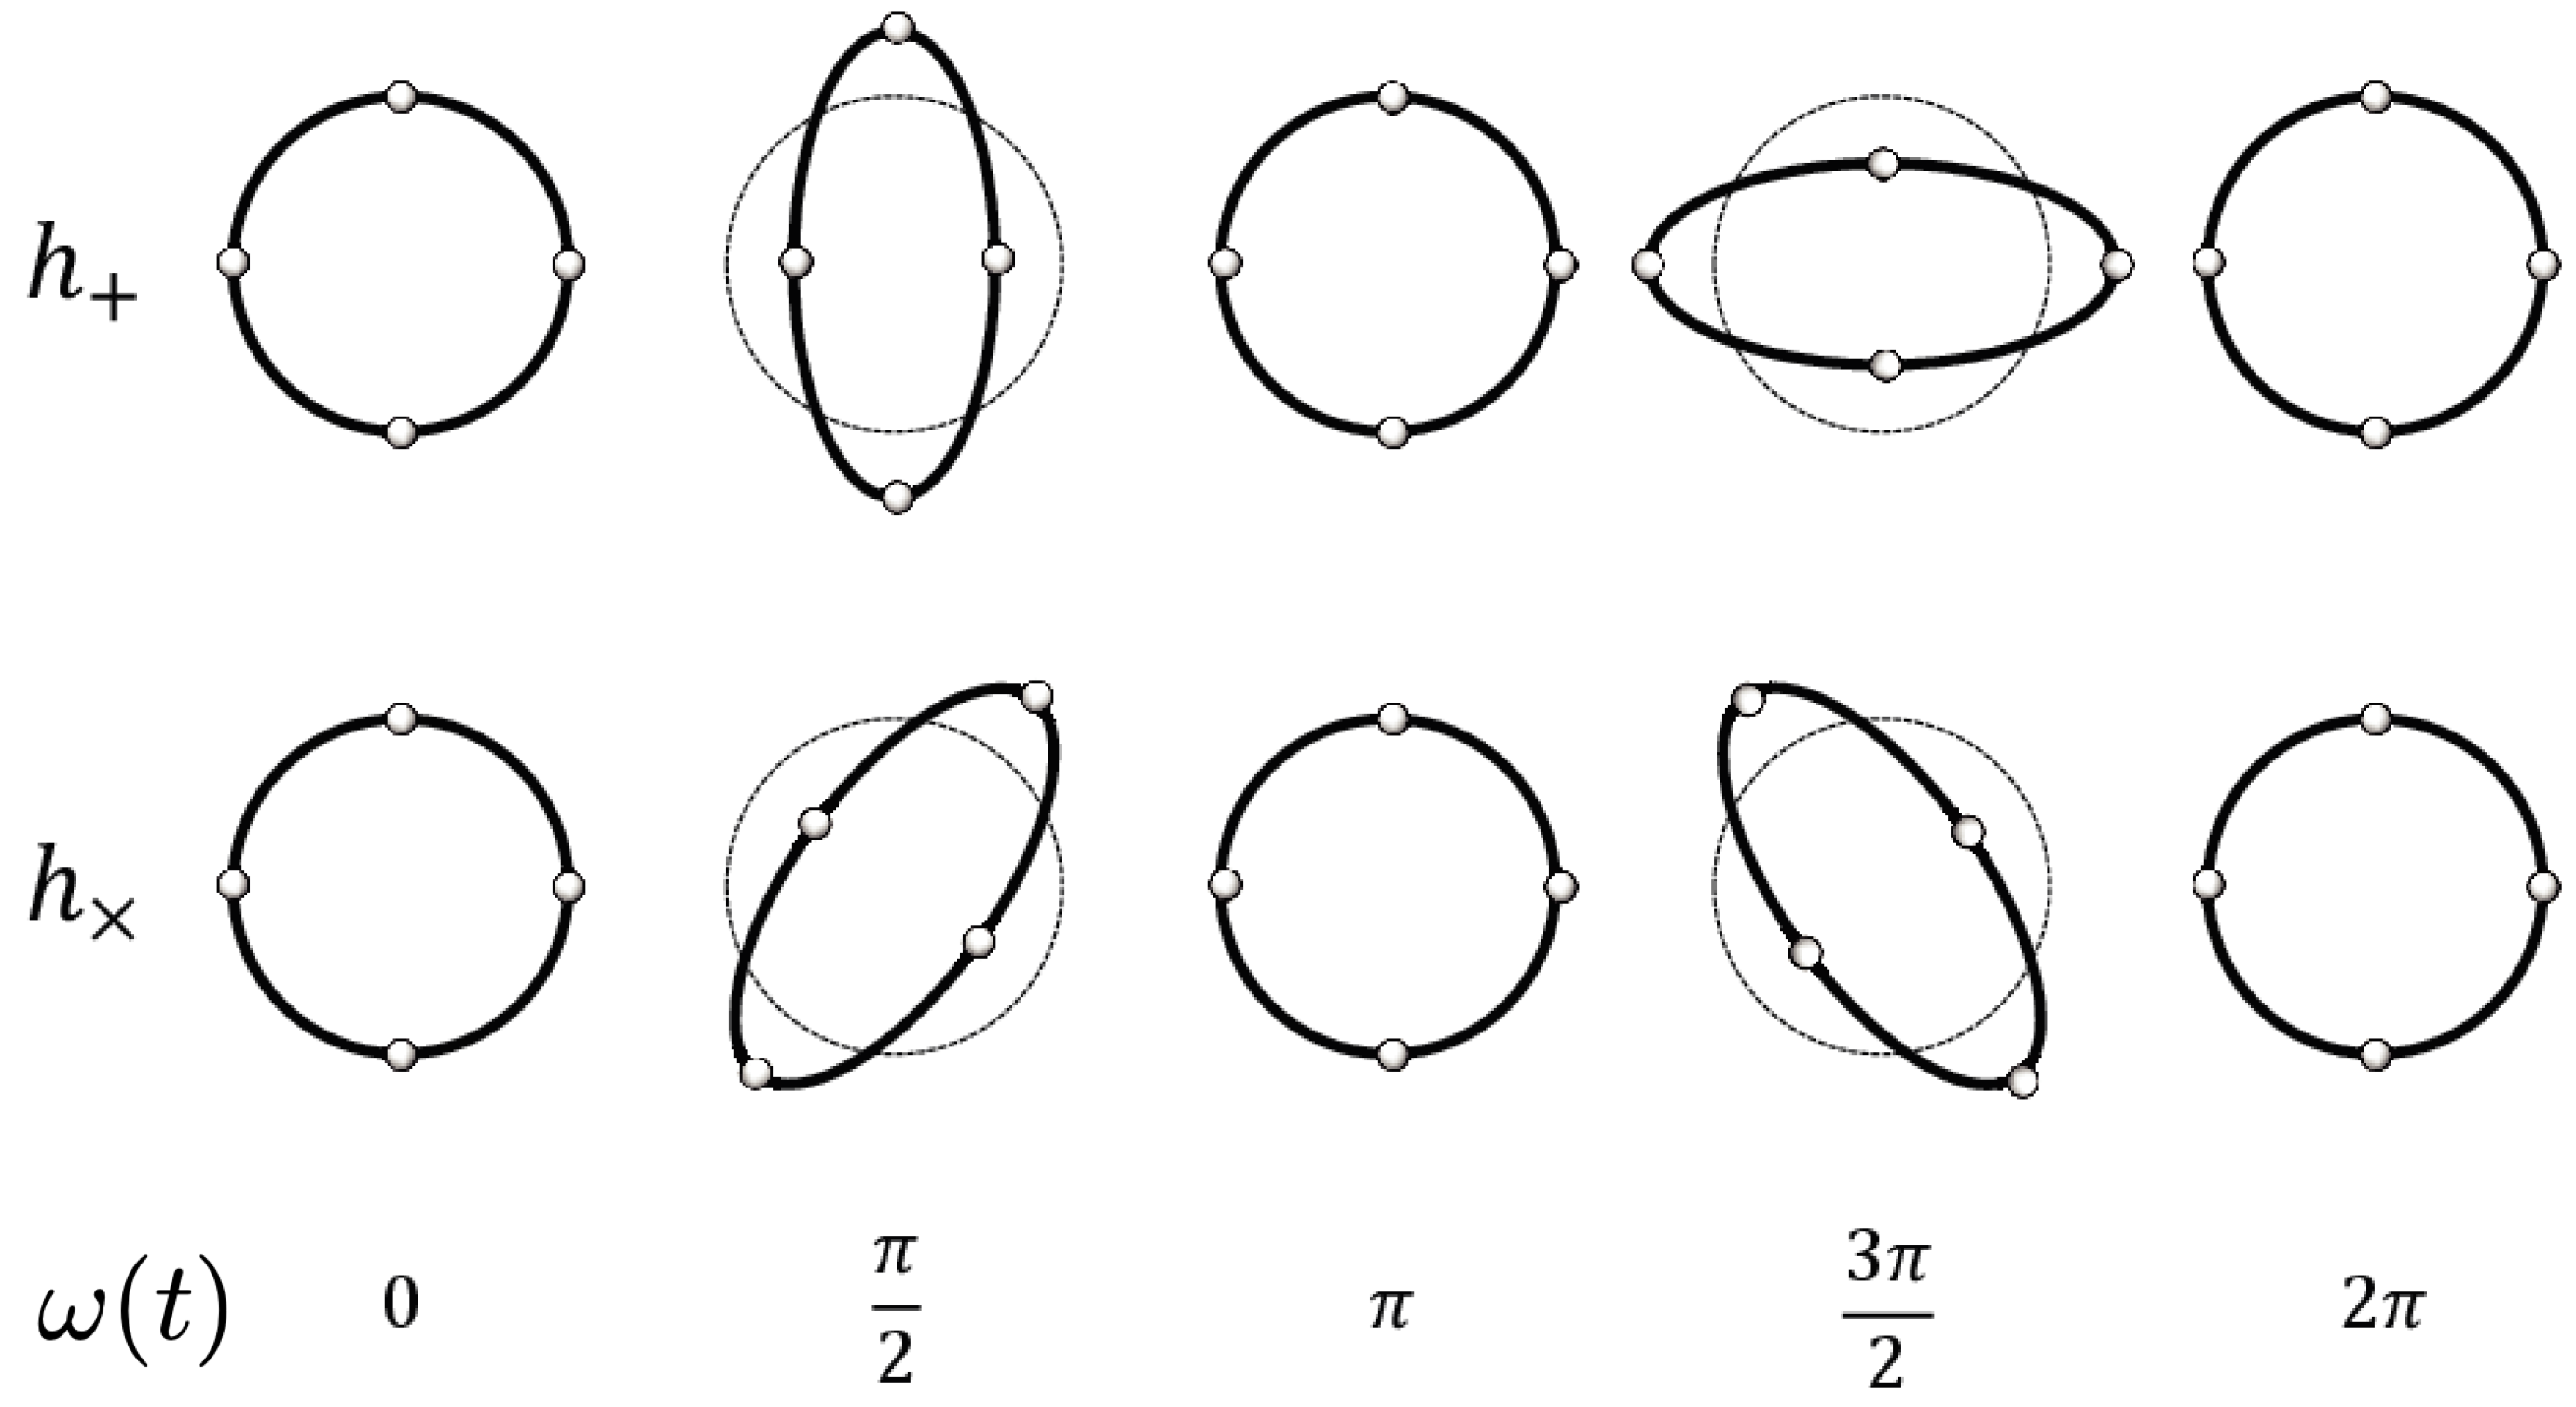
\includegraphics[scale=1]{ring}
\centering
\caption{The effects of plus and cross polarization on a ring of test masses. The plus polarization alternately compresses and stretches the x- and y-separations. 
The cross polarization has the same effect only rotated by  $\ang{45}$.}
\label{fig:ring}
\end{figure}




\subsection{Energy and momentum of gravitational waves}

 Energy has been one of the most confusing aspects of gravitational wave theory and hence of general relativity.
The fact that GWs do indeed carry energy and momentum is already clear from the discussion of the interaction of GWs with test masses: 
in the proper detector frame, an incoming GW sets in motion a ring of test masses initally at rest, so GWs impart kinetic energy to these asses. 
If, for example, these masses are connected together with a loose spring with friction, this kinetic energy will be dissipated into heat. 
Conservation of energy requires that the kinetic energy acquired by the test masses must necessarily come from the energy of the GWs. 
The problem is difficult because of the equivalence principle: in a local frame there are no waves and hence no local definition of energy that can be coordinate-invariant. 
Moreover, a wave is a time-dependent metric, and in such spacetimes there is no global energy conservation law. (Recall that conservation laws are associated with symmetry. 
Angular momentum is conserved only in axisymmetric systems, or in systems governed by axisymmetric forces or fields. 
Likewise, energy is conserved on in time-invariant systems.) Energy is only well-defined in certain regimes, which coincide with those for which waves can be cleanly separated from ”background”
 metrics.

\subsection{Effect of gravitational waves on the background spacetime}
In order to consider the fact that GWs generate a curvature, the background spacetime has to be dynamical, and this implies that GWs are defined as perturbations over some curved, dynamical, background metric $\bar g_{\mu \nu}$, that is now allowed to be curved and expand in such way
\begin{equation}
g_{\mu \nu}(x) = \bar g_{\mu \nu}(x) + h_{\mu \nu}(x) \hspace*{2cm}\|h_{\mu\nu}\|\ll 1
\end{equation}
In order to understand how the perturbation $h_{\mu \nu}$ propagates and how it affects the background spacetime, we have to to decide which part of $g_{\mu\nu}$ is the background and which is the fluctuations. Having a dynamical background metric requires a splitting that in linearized theory, having chosen the background metric as the constant flat-space metric $\eta_{\mu\nu}$, was not necessary.

There is no natural way to do such a split, hence some assumptions are needed: we are considering the situation in which, in some reference frame, we can separate the metric into a background plus fluctuations, and this separation is based on the fact that there is a clear distinction of scales either in space or in time.  
Assuming that in some coordinate system, the $\bar g_{\mu \nu}$ has some typical length scale of spatial variation $L_B$, on top of which small amplitude perturbations are superimposed, characterized by a wavelength $\lambda$ such that $\lambda \ll L_B$. In this case $h_{\mu\nu}$ has the physical meaning of small ripples on a smooth background. 
Equivalently, in a frequency space $\bar g_{\mu\nu}$ has frequencies up to a maximum value $f_b$ and  $h_{\mu\nu}$  is peaked around a frequency $f$, with $f >> f_b$.

First of all, let's expand the Einstein equations around the background $\bar g_{\mu \nu}$ in terms of two small parameters: the typical amplitude $h= O(|h_{\mu\nu}|)$, and either $\lambda/L_B$ or $f_B/f$. 
It is convenient to write the Einstein equations as 
\begin{equation}
R_{\mu\nu} = {{8\pi G}\over c^4}(T_{\mu\nu}- {1 \over 2}g_{\mu\nu}T) 
\end{equation}
where $T_{\mu\nu}$ is the energy-momentum tensor of matter and $T$ its trace.The expantion of the Ricci tensor to $O(h^2)$ is
\begin{equation}
R_{\mu\nu} = {\bar R_{\mu\nu}} + R_{\mu\nu}^{(1)} + R_{\mu\nu}^{(2)} + ...
\end{equation}
where $ {\bar R_{\mu\nu}}$ is constructed with $\bar g_{\mu\nu}$ only, thus it contains only low frequency modes;
$R_{\mu\nu}^{(1)}$ is linear in $h_{\mu\nu}$ and it contains high frequency modes;
and $R_{\mu\nu}^{(2)} $ is quadratic in $h_{\mu\nu}$, it contains both high and low frequency modes.
Therefore the Einstein equations can be split into two separate equations for the low and high frequency parts
\begin{equation}
{\bar R_{\mu\nu}} = -[R_{\mu\nu}^{(2)}]^{Low} + {{8\pi G}\over c^4}(T_{\mu\nu}- {1 \over 2}g_{\mu\nu}T) ^{Low}
\end{equation}
and
\begin{equation}
 R_{\mu\nu}^{(1)} = - [R_{\mu\nu}^{(2)}]^{High} +  {{8\pi G}\over c^4}(T_{\mu\nu}- {1 \over 2}g_{\mu\nu}T)^{High}
\end{equation}
One way to project on the long wavelenght modes is to introduce a scale $\bar l$ such that $\lambda << \bar l << L_B$, and averaging over a spatial volume with side $\bar l$.
A wavelenght of order $L_B$ is constant over the volume used for the averaging, while modes with a reduced wavelenght of order $\lambda$ are oscillating very fast and average to zero. 
The low-frequency Einstein equations become
\begin{equation}
 {\bar R_{\mu\nu}} = - <R_{\mu\nu}^{(2)}> +  {{8\pi G}\over c^4}(T_{\mu\nu}- {1 \over 2}g_{\mu\nu}T) ^{High}
\end{equation}
where $<..>$ denotes a spatial average over many reduced wavelenghts, over a volume with sides $l$.
We now define an effective energy-momentum tensor of matter, $\bar T^{\mu\nu}$ 
\begin{equation}
{\bar T^{\mu\nu}} - {1 \over 2}{\bar g_{\mu\nu}}{\bar T} = <T_{\mu\nu}- {1 \over 2}T>
\end{equation}
where ${\bar T}$ is the trace. 
We also define the quantity $t_{\mu\nu}$ as
\begin{equation}
t_{\mu\nu} = -{{c^4}\over{8\pi G}}<R_{\mu\nu}^{(2)} - {1 \over 2}{\bar g_{\mu \nu}}R^{(2)}>
\end{equation}
whose trace is $t= {\bar g^{\mu\nu}}t_{\mu\nu} = {{c^4}\over{8\pi G}}<R_{\mu\nu}^{(2)}>$.
Then the low-frequency Einstein equations can be written as
\begin{equation}
 {\bar R_{\mu\nu}} = -{1 \over 2}{\bar g^{\mu\nu}} {\bar R} =  {{8\pi G}\over c^4}({\bar T_{\mu\nu}}+t_{\mu\nu})
\end{equation}
These equations determine the dynamics of $\bar g_{\mu\nu}$, which is the long-wavelength part of the metric, in terms of the low-frequency part of the matter energy-momentum tensor, $\bar T_{\mu\nu}$, and of a tensor $t_{\mu\nu}$ which does not depend on the external matter but only on the gravitational field itself, and is quadratic in $h_{\mu\nu}$.
These equations show that the effect of GWs on the background curvature is formally identical to that of matter with energy-momentum tensor $t_{\mu\nu}$, which comes out automatically in an averaged form because one is passing from a microscopic description to a macroscopic one.

\subsection{The energy-momentum tensor of GWs}
Both $h_{\mu\nu}$ and $\bar g_{\mu\nu}$ have 10 degrees of freedom, out of which 8 are gauge modes and 2 are physical modes, hence $t_{\mu\nu}$ must have contributions due to physical modes, which will give the energy-momentum tensor of the GWs, and describe physical effects that cannot be gauge away, and gauge modes, which are due to the choice of the coordinate system and can be made to vanish with an appropriate gauge choice.

This simplifies greatly within spatial average because space time derivative $\partial_\mu$ can be integrated by parts, neglecting boundary term. Using this together with $\partial^{\mu} h_{\mu\nu}$, $h=0$, $\square h_{\alpha \beta} = 0$, one finds
\begin{equation}
<R^{(2)}_{\mu\nu}> = -{1 \over 4}<{\partial_{\mu}h_{\alpha\beta}h^{\alpha\beta}}> 
\end{equation}
while
\begin{equation}
<R^{(2)}> = 0
\end{equation}
because it vanishes upon integration by parts and using the equation of motion ${\square h_{\alpha\beta}}=0$.
With these simplifications, the energy-momentum tensor associated with gravitational waves becomes
\begin{equation}
t_{\mu\nu} = {c^4 \over {32\pi G}}<\partial_{\mu}h_{\alpha\beta}\partial_{\nu}h^{\alpha\beta}>
\end{equation}
it can be verified that the expression is gauge invariant (but not without the spatial averaging), the total energy-momentum is covariantly conserved: $\nabla^{\mu}(\bar{T_{\mu\nu}}+t_{\mu\nu})=0$.
Because of gauge invariance, $h_{\mu\nu}$ can be replaced with metric perturbation in TT gauge.
The gauge invariant energy density in gravitational waves is:
\begin{equation}
t^{00} = {c^2\over{32\pi G}}<\dot{h_{ij}^{TT}}\dot{h_{ih}^{TT}}>
\end{equation}
For the special case of a plane wave propagating in the $z$ direction, the stress-energy tensor has only three non-zero components, which take the simple form
\begin{equation}
t^{00} = {t_{zz}\over c^2}= -{t_{0z}\over c}= {c^2\over{16\pi G}}<\dot{h_{+}^2}+\dot{h_{\times}^2}>
\end{equation}
where $t_{00}$ is the energy density, $t_{zz}$ is the momentum flux and $t_{0z}$ the energy flow along the $z$ direction per unit area and unit time. 
Similarly momentum density is:
\begin{equation}
t^{0k} = -{c^2\over{32\pi G}}<\dot{h_{ij}^{TT}}\partial^k{h_{ih}^{TT}}>
\end{equation}


It is now straightforward to compute the energy flux associated to the energy-momentum tensor starting from the conservation of the $t_{\mu\nu}$.
The energy contained in a spatial volume $V$ bounded by a large sphere $S$ of radius $r$ will be:
\begin{equation}
E_{V} = \int_{V} d^3x t^{00}
\end{equation}
Thus the energy emitted in gravitational waves from the source is: 
\begin{equation}
{{dE_{GW}}\over {dt}} = - \int_{V} d^3x \partial_t t^{00}
\end{equation}
and the energy passing through the sphere $S$ per unit time at a large distance from the source is:
\begin{equation}
{{dE_{GW}}\over {dt}} = {{c^3r^2}\over{16\pi G}}\int_{S} d\Omega<\dot{h_{+}^2}+\dot{h_{\times}^2}>
\end{equation}
The energy flux has all the properties one would anticipate by analogy with electromagnetic waves: it is conserved (the amplitude dies out as $1/r$, the flux as $1/r^2$), it can be absorbed by detectors, and it can generate curvature like any other energy source in general relativity. 
Similarly for momentum of the GWs inside a spherical shell V at large distances from the source is given by:
\begin{equation}
{{dP^{k}_{GW}}\over{dt}} = -{{c^3r^2}\over{32\pi G}}\int_{S}d\Omega<\dot{h_{ij}^{TT}}\partial^k{h_{ih}^{TT}}>
\end{equation}

 
\subsection{Generation of gravitational waves}
A GW is produced by coherent bulk motions of huge amounts of mass. 
Similarly to the well known fact that accelerating charges produce EWs, in quite general terms accelerating masses can produce GW.
First we consider the field of a source in linearized theory and we use a slow-motion approximation to compute the radiated field, the linear wave equation can be solved using the standard formula for retarded potentials. 

The Einstein equation in linearized theory are:
\begin{equation}
\square {\bar h_{\mu\nu}} = - {{16 \pi G}\over c^4} T_{\mu\nu}
\end{equation}
Its general solution is the following retarded integral for the field at a position $x$ and a time $t$ in terms of the source at a position $x\prime$ and the retarded time:
\begin{equation}
 {\bar h_{\mu\nu}} (t, x) = {{4G}\over c^4} \int d^3x\prime {1 \over {|x-x\prime|}} T_{\mu\nu}(t-{{|x-x\prime|}\over c}, x\prime)
\end{equation}
Unlike in Newtonian gravity, the gravitational field at a point $(ct,x)$ is only influenced by the matter source at the retarded times $t\prime \equiv t−\|x-x\prime\|/c$, the lag resulting from the time needed for a signal propagating at the speed of light $c$ to get from a point $x\prime$ inside the source to the point $x$. 
Let us suppose that the origin of coordinates is in or near the source, and the field point $x$ is far away: setting $|x-x\prime|= r$, we take the limit $r \longrightarrow \infty$ at fixed $t$. 
Assuming in addition that the source is $slowly varying$, in the sense that its energy-momentum tensor does not vary much over a light-crossing time, standard manipulations yield for the field in the radiation zone
\begin{equation}
{\bar h_{\mu\nu}} (t, x) = {{4G}\over {c^4r}} \int d^3x\prime  T_{\mu\nu}(t-{r\over c}, x\prime)
\end{equation}
where $r = \|x\|$ is the distance from the source, and we have expanded the term $|x-x\prime|$ in terms of $x\prime$. The lowest order is r, and all higher order terms are smaller than this by powers of $r^-1$. Therefore, they contribute terms to the field that fall  off faster than $1/r$, and they are negligible in the far zone. So we can simply replace $|x-x\prime|$ by $r$, and take it out of the integral. 
Now expanding $t−\|x-x\prime\| = t - r + n^i x\prime_i + O(1/r)$, the terms of order $1/r$ are negligible for the same reason as above, but the first term in this expansion must be taken into account. It depends on the direction to the field point, given by the unit vector $n^i$. We use this by making a Taylor expansion in time on the time-argument of the source. The combined effect of these approximations is 
\begin{equation}
{\bar h_{\mu\nu}} = {4 \over r} \int {d^3x\prime [T_{\mu\nu}(t\prime, x\prime) + T_{\mu\nu,0}(t\prime,x\prime)n^ix\prime_i + {1\over2}T_{\mu\nu,00}(t\prime,x\prime)n^in^jx\prime_i x\prime_j + ....]}
\end{equation}
The integrals in the above expression contain multipole moments of the source, defined in analogy to electrodynamics, with the charge density replace by the energy density $T_{00}$.
The monopole moment is defined as
\begin{equation}
M(t\prime) = \int d^3x\prime T^{00}(t\prime, x\prime)
\end{equation}
while the dipole moment is
\begin{equation}
D_j(t\prime) = \int d^3x\prime T^{00}(t\prime, x\prime)x\prime_j
\end{equation}
Finally, the moment of inertia of the source:
\begin{equation}
I_{jk}(t\prime) = \int d^3x\prime T^{00}(t\prime, x\prime)x\prime_jx\prime_k
\end{equation}
The radiative degrees of freedom are contained in the spatial part of the metric, so we by combining ${\bar h_{\mu\nu}}$ with $\partial_{\mu} T^{\mu\nu}$, the spatial components of ${\bar h_{\mu\nu}}$ are given by

\begin{equation}
{\bar h_{ij}(t, x)} = {{2G}\over{c^4r}} {\ddot I_{ij}}(t\prime)
\end{equation}
We are already in Lorentz gauge, but we  are manifestly not in $TT$ gauge: applying this gauge to themass quadrupole field eliminates the momentum part of the field, and renders the time component of the field constant. Since waves are time-dependent, the time-dependent part of the field is now purely spatial, transverse and traceless.
 
The expression for the spatial part of the field can be seen by constructing the trace-free part of the tensor $I_{jk}$, defined as the source's $mass quadrupole moment$:
\begin{equation}
Q_{jk}(t) = \int d^3x \rho(t, x) (x_i x_j - {1 \over 3}\|x\|^2 \delta_{ij})  
\end{equation}
where $\rho$ is the matter density in a volume element $d^3x$ at the position $x^i$.
To obtain the metric perturbation in the $TT$ gauge, it is enough to consider the transverse-traceless part of ${\bar h_{ij}}$, and this is achieved by means of an appropriate projection:
\begin{equation}
 h_{ij}^{TT}(t, x) = {{2G}\over{c^4r}}  \lambda_{ij,kl}(n){\ddot Q_{kl}}(t\prime)
\end{equation}
This result show that, to leading order in a multipolar expansion, gravitational waves are generated by any time-varying quadrupole moment.
The only property of the source that a gravitational wave detector can measure far away from the source is, thus, the second time derivative of the quadrupole moment at a retarded time. 
The laws of conservation of mass and linear momentum forbid the emission of monopolar or dipolar gravitational radiation.
In this sense, gravitational radiation is quadrupole radiation, while in electromagnetism while the electric charge (the monopole) is conserved, the electric dipole moment is not, so electromagnetic radiation is predominantly dipolar.



\chapter{Modeling formalism}
\section{Post-Newtonian (PN) theory}
\section{Numerical relativity}
\section{Perturbation theory}


\chapter{Gravitational Waves Data analysis}
\section{Template Banks}
\section{Matched Filter}
\section{Interferometer noise curve}
\section{Signal-to-noise ratio}

\chapter{Electromagnetic radiation from binary black hole - neutron star systems}
\section{Accretion disks around black holes: dynamical evolution}
\section{Short gamma-ray bursts}
\section{} 





\backmatter
\cleardoublepage

\phantomsection % Give this command only if hyperref is loaded \addcontentsline{toc}{chapter}{\bibname}

\begin{thebibliography}{100}
   \bibitem[nome]{riferimento}
\end{thebibliography}

\end{document} 

